%%% File encoding: UTF-8
%%% äöüÄÖÜß  <-- keine deutschen Umlaute hier? UTF-faehigen Editor verwenden!

%%% Magic Comments zum Setzen der korrekten Parameter in kompatiblen IDEs
% !TeX encoding = utf8
% !TeX program = pdflatex 
% !TeX spellcheck = de_DE
% !BIB program = biber

\documentclass[bachelor,german]{hgbthesis}
% Zulässige Optionen in [..]: 
%   Typ der Arbeit: diploma, master (default), bachelor, internship 
%   Hauptsprache: german (default), english
%%%----------------------------------------------------------

\RequirePackage[utf8]{inputenc}		% bei der Verw. von lualatex oder xelatex entfernen!

\graphicspath{{images/}}    % Verzeichnis mit Bildern und Grafiken
\logofile{logo}				% Logo-Datei = images/logo.pdf (\logofile{}, wenn kein Logo gewünscht)
\bibliography{references}  	% Biblatex-Literaturdatei (references.bib)
%%%----------------------------------------------------------
% Angaben für die Titelei (Titelseite, Erklärung etc.)
%%%----------------------------------------------------------

%%% Einträge für ALLE Arbeiten: -----------------------------
\title{Emacs für die moderne Hardware- und Software-Entwicklung}
\author{Thomas \ Reisinger} \programname{Hardware-Sotware Design}
\placeofstudy{Hagenberg im Mühlkreis} \dateofsubmission{2018}{09}{10}
% {YYYY}{MM}{DD}

%%% Zusätzlich für eine Bachelorarbeit: ---------------------
\thesisnumber{1510306033-A}   % Stud-ID, z.B. 1310238045-A  
% (A = 1. Bachelorarbeit)
\semester{Sommersemester 2018} 
\coursetitle{Bachelorseminar} 
\advisor{FH-Prof. DI. Markus Pfaff}

%%% Restriktive Lizenformel anstatt CC (nur für Typ master) -
%\strictlicense

%%%----------------------------------------------------------
\begin{document}
%%%----------------------------------------------------------

%%%----------------------------------------------------------
\frontmatter                    % Titelei (röm. Seitenzahlen)
%%%----------------------------------------------------------

\maketitle
\tableofcontents

\chapter{Kurzfassung}
\label{cha:kurzfassung}
Als Hardware- und Software-Entwickler/in ist es üblich, eine große
Anzahl an Entwicklungsumgebungen für einzelne Programmiersprachen zu
verwenden. Häufig findet die Beschreibung der Hardware oder die
Implementierung der Software auf unterschiedlichen Betriebssystemen
statt. Dadurch kommen in vielen Fällen noch weitere
Entwicklungsumgebungen hinzu. Damit diese Aufgaben mit einer einzigen
Software bewältigt werden können, wird der Editor Emacs
vorgestellt.\\\\ Diese Arbeit beschreibt, wie Emacs als Alternative
für die Hardware- und Software-Entwicklung eingesetzt werden
kann. Dafür wird Emacs spezifisch an die Anforderungen eines Hardware-
und Software-Entwicklers angepasst. Im Zuge der Arbeit wird
beschrieben, wie diese Anpassungen durchgeführt werden. Die
Konfigurationen setzten Emacs als eigenständige Entwicklungsumgebung
für die Sprachen C, C++, Emacs Lisp, Latex, Python und VHDL auf. Zur
Realisierung werden Pakete verwendet, welche von der Community zur
Verfügung gestellt werden. Die Funktionalität und Konfiguration aller
verwendeten Pakete werden beschrieben. Für diese Pakete werden eigene
Funktionen implementiert, damit die Funktionalität der Pakete für
mehrere Sprachen möglichst einfach genutzt werden kann.\\\\ Es werden
ebenfalls Pakete vorgestellt, welche in Emacs eine grafische
Oberfläche implementieren. Mit diesen grafischen Paketen sieht Emacs
ansprechender aus. Dadurch wird Personen, die grafische Oberflächen
bevorzugen, Emacs für die Hardware- und Software-Entwicklung
schmackhaft gemacht. Damit auch Emacs-Neulingen ein einfacher Einstieg
ermöglicht wird, werden die Grundlagen von Emacs beschrieben.\\\\ In
der Arbeit werden Beispiele von Workflows für die einzelnen
Programmiersprachen beschrieben. Dadurch kann Emacs als
Entwicklungsumgebung schnell und einfach in den Alltag eine/s/r
Hardware- und Software-Entwickler/s/in integriert werden.\\
		
\chapter{Abstract}

\begin{english} %switch to English language rules
Hardware and software engineers are often confronted by many different
integrated development environments. That big amount of environments
exists because in most cases there is one development environment for
each programming language. Very often engineers have to develop their
hardware and software on different operating systems. That adds more
environments to their list. To avoid this big amount of development
environments, Emacs will be introduced as an alternative.\\\\ This
thesis describes how Emacs can be used for hardware and software
development. Emacs requires to be configured specifically to the needs
of hardware and software engineers. It will be described, how the
Emacs configuration works. The configuration in this thesis modifies
Emacs for the use as an integrated development environment for the
programming languages C, C++, Emacs Lisp, Python and VHDL. In the
configuration file, there are packages offered by the Emacs
community. The functionality and configuration of all packages are
described. There are some additional functions implemented to offer a
simpler and quicker usage for the functionality of these
packages. Some packages add graphical user interface elements to
Emacs. These packages should animate people for the use of Emacs, that
are more likely to develop on graphical environments. Emacs is
introduced from scratch, especially for people who are completely new
to Emacs.\\\\ The thesis describes some possible workflows for the
development with different programming languages. This is meant to
offer software and hardware developers an easier and quicker access to
Emacs. That way it should be easy for them, to include Emacs in their
daily workflow.
\end{english}

			

%%%----------------------------------------------------------
\mainmatter          % Hauptteil (ab hier arab. Seitenzahlen)
%%%----------------------------------------------------------

\chapter{Einleitung}
Dieses Kapitel gibt einen Überblick über die Inhalte und
Rahmenbedingungen der Arbeit.
\label{cha:Einleitung}
\section{Motivation}
Als Hardware- Software-Entwickler/in wird man im Alltag mit einer
Vielzahl an Programmiersprachen konfrontiert. Ebenfalls reicht ein
einziges Betriebssystem nicht aus, um alle Aufgaben der Arbeitswelt zu
bewältigen. Hinzu kommt noch, dass meist eigene Programme zur
Versionsverwaltung und für die Erstellung von technischen Dokumenten
benötigt werden.

Es gibt einige Möglichkeiten, um diese Vielzahl an Programmiersprachen
auf unterschiedlichen Betriebssystemen zu verwalten. Die erste ist,
für jede Programmiersprache auf jedem Betriebssystem eine eigene
Entwicklungsumgebung zu verwenden. Damit ein effektives Arbeiten
gewährleistet werden kann, muss jede dieser Entwicklungsumgebungen gut
beherrscht werden. Die zweite Möglichkeit ist, einen einfachen Editor
zu wählen, welches auf allen Betriebssystemen installiert ist. Durch
diese einfachen Textverarbeitungsprogramme ist man in vielen Fällen
dazu gezwungen, auf wichtige Features, welche integrierte
Entwicklungsumgebungen mitbringen, zu verzichten. Die dritte
Möglichkeit, welche in dieser Arbeit vorgestellt wird, ist die
Kombination aus den ersten beiden Möglichkeiten. Die Verwendung eines
Editors, welcher auf einer Vielzahl an Betriebssystemen verfügbar
ist. Jedoch muss auf Features wie automatische Vervollständigung,
Syntax-Hervorhebung und Syntax-Überprüfung nicht verzichtet werden.

Bei der Auswahl eines solchen Editors sollte darauf geachtet werden,
dass eine große \textit{Community} dahinter steht. Dadurch müssen die
meisten Anpassungen nicht komplett selbst programmiert werden und es
kann auf Paketen der \textit{Community} aufgebaut werden. Aus diesen
Gründen wird \textit{GNU
  Emacs}\footnote{\url{https://www.gnu.org/software/emacs/}}
gewählt.

Die Konfiguration von Emacs, welche Grundvoraussetzung ist, um Emacs
effektiv in den täglichen Workflow einbinden zu können, erweist sich
meist als sehr aufwändig. Außerdem werden viele Personen durch die
Vielzahl an Tastenkombinationen abgeschreckt. Aus diesem Grund wird
der Einstieg in Emacs oft gemieden, wodurch der Ansporn für diese
Arbeit entstanden ist.\\

\section{Ziel der Arbeit}
Ziel ist es, Informatik-Studierenden einen einfachen Einstieg in Emacs
als Entwicklungsumgebung für mehrere Programmiersprachen zu
ermöglichen. Um dies zu erreichen, werden fertige
Konfigurationsdateien zur Verfügung gestellt und erklärt. Außerdem
wird die Verwendung dieser Konfigurationsdateien beschrieben. Emacs
soll eine alternative zu herkömmlichen Entwicklungsumgebungen bieten,
um ein effektives Arbeiten zu ermöglichen. Damit dies erreicht werden
kann, richten diese Konfigurationsdateien Emacs als vollwertige
Entwicklungsumgebung für diverse Programmiersprachen ein. Diese
Programmiersprachen sind C, C++, Emacs Lisp, Python und VHDL. Die
Konfiguration soll auf mehreren Betriebssystemen lauffähig sein.\\

\section{Gliederung}
Im Kapitel \ref{cha:sw-entwicklung} wird die übliche Vorgehensweise
von Hardware-Software-Entwickler/n/innen dargestellt und welche
Probleme diese mit sich bringen kann. In diesem Kapitel wird ebenfalls
beschrieben wann sich ein Umstieg auf Emacs lohnen kann und wann
nicht. Im Kapitel~\ref{cha:grundlagen} folgt eine Einführung in die
Grundlagen von Emacs. In diesem Kapitel wird auch die Installation von
Emacs auf unterschiedlichen Betriebssystemen behandelt. Im Kapitel
\ref{cha:pakete} werden alle verwendeten Pakete und ihre Funktion
beschrieben. Das Kapitel \ref{cha:Konfiguration} handelt von den
Konfigurationsdateien. Es werden die unterschiedlichen
Konfigurationsdateien erläutert. Im Kapitel \ref{cha:workflow} wird
ein einfacher Workflow für die einzelne Programmiersprachen
beschrieben. Dieses Kapitel soll Emacs-Neulingen ermöglichen, Emacs
direkt in den alltäglichen Workflow einzubauen.\\

\chapter{Gegenüberstellung}
\label{cha:sw-entwicklung}
Dieses Kapitel stellt die Ausgangslage als Hardware- und
Software-Entwickler/in dar. Es wird beschrieben, in welchen Fällen
sich ein Umstieg auf Emacs lohnt.

\section{Herkömmliche Entwicklungsumgebungen für unterschiedliche Aufgaben}
In den folgenden Abschnitten werden übliche Entwicklungsumgebungen für
Hardware- und Software-Entwickler/innen aufgelistet. Im Anschluss
werden die möglichen Probleme, die diese Vielzahl an
Entwicklungsumgebungen mit sich bringen kann, zusammengefasst.\\

\subsection{Entwicklungsumgebungen zur Erstellung von Dokumenten}
In der Informatik werden einige Programme benötigt, um ein Projekt
effektiv ausarbeiten zu können. Zunächst wird eine Software für die
Erstellung technischer Dokumente benötigt. Diese Dokumente reichen von
Pflichtenheften bis hin zu Softwarebeschreibungen. Dafür eignet sich
die Sprache LaTeX, ein Editor für LaTeX ist zum Beispiel
\textit{MikTex}\footnote{\url{https://miktex.org/}}. Eine weitere
Optionen ist Software aus dem Paket \textit{Microsoft
  Office}\footnote{\url{https://www.office.com/}}, wie
\textit{Microsoft
  Word}\footnote{\url{https://products.office.com/de-at/word}} oder
\textit{Microsoft
  Excel}\footnote{\url{https://products.office.com/de-at/excel}} für
die Erstellung von Tabellen.\\

\subsection{Entwicklungsumgebung zum Entwickeln von Code}
Als nächstes wird eine Entwicklungsumgebung für die jeweils verwendete
Programmiersprache ausgewählt. Eine kostenlose Variante ist
\textit{Eclipse}\footnote{\url{https://www.eclipse.org/}}. Es kann
aber auch eine Version von \textit{Visual
  Studio}\footnote{\url{https://visualstudio.microsoft.com/}}
verwendet werden. Es muss bei der Wahl der Entwicklungsumgebung auf
folgende Punkte geachtet werden:
\begin{itemize}
\item Auf welchem Betriebssystem wird entwickelt.
\item Für welche Plattform wird entwickelt.
\item Welche Programmiersprache wird verwendet.
\item Wenn mehrere Programmiersprachen zum Einsatz kommen, muss eine
  Entwicklungsumgebung gefunden werden, die all diese Sprachen
  unterstützt. Andernfalls müssen mehrere Umgebungen verwendet werden.
\item Unterstützt die Entwicklungsumgebung den erforderlichen
  Compiler.
\end{itemize}

\subsection{Sonstige zusätzliche Software}
Zur Versionsverwaltung wird in einigen Fällen eine grafische
Oberfläche bevorzugt. Für Versionsverwaltungssysteme wie
\textit{Git}\footnote{\url{https://git-scm.com/}} und
\textit{Subversion}\footnote{\url{https://subversion.apache.org/}}
gibt es zum Beispiel \textit{Tortoise
  Git}\footnote{\url{https://tortoisegit.org/}} und \textit{Tortoise
  SVN}\footnote{\url{https://tortoisesvn.net/}}.\\

\subsection{Probleme bei einer großen Anzahl an Software}
Wird an einem Projekt für einen großen Zeitraum gearbeitet und für
dieses Projekt wurden eine oder zwei Entwicklungsumgebungen
ausgewählt. Dann ist nichts dagegen einzuwenden, diese
Entwicklungsumgebungen zu erlernen und zu verwenden. Jedoch gibt es
ebenfalls Projekte, die nur von kurzer Dauer sind. Es muss jeder
persönlich abschätzen, ob es Sinnvoll ist eine neue
Entwicklungsumgebung für diesen kurzen Zeitraum zu erlernen.

Ebenfalls kann es vorkommen, dass für die Entwicklung einiger
Abschnitte des Projektes ein Server zur Verfügung gestellt wird, auf
welchem eine Distribution von
\textit{Linux}\footnote{\url{https://www.kernel.org/}} läuft. Dies ist
problematisch, wenn die persönliche Wahl der Entwicklungsumgebung auf
eine Windows-basierte Entwicklungsumgebung fiel und diese für Linux
nicht verfügbar ist. So muss wieder eine neue Entwicklungsumgebung für
die erforderliche Aufgabe gesucht und erlernt werden. Andernfalls muss
man sich mit einem einfachen Editor zufrieden geben. Weiter Probleme
können auftreten, wenn Programmierer am selben Projekt auf
unterschiedlichen Betriebssystemen arbeiten. In einigen Fällen hat man
selber auch gar keine Wahl, welche Entwicklungsumgebung zu verwenden
ist. Zum Beispiel wenn man einem Projekt zugewiesen wird, für das eine
Entwicklungsumgebung bereits gewählt wurde. Hier kann wiederum auf
einen einfachen Editor ausgewichen werden oder man lernt, mit der
Entwicklungsumgebung zu arbeiten.\\

\section{Warum Emacs}
Emacs ist einer der mächtigsten Editoren und eine eigenständige
Arbeitsumgebung. Damit ist gemeint, dass Emacs auch Dateien
umbenennen, verschieben, kopieren und löschen kann. Wenn Emacs in
einer grafischen Umgebung gestartet wird, können grafische Objekte wie
Bilder angezeigt werden. Wird Emacs in einem Terminal ausgeführt, so
kann zwar nur Text angezeigt werden, aber Emacs kann so auch auf einem
Server ohne grafischer Oberfläche verwendet werden. Emacs ist ein
Emacs, welches jedoch in einem Programmiergerüst einem so genanntem
{\glqq}Framework{\grqq} läuft. Dieses Programmiergerüst ist höchst
personalisierbar, wodurch integrierte Entwicklungsumgebungen
geschaffen werden können, die an die eigenen Bedürfnisse angepasst
sind. Wird Emacs unter
\textit{Unix}\footnote{\url{http://www.opengroup.org/unix}} verwendet,
so können alle \textit{Unix}-Kommandos innerhalb von Emacs ausgeführt
werden. Das selbe gilt auch für
\textit{Mac-OS}\footnote{\url{https://www.apple.com/at/macos/high-sierra/}}
und \textit{Windows}. Es ist dabei zu beachten, dass die
\textit{Windows}-Kommandozeile bei weitem nicht so mächtig ist, wie
die \textit{Unix}-Kommandozeile. Die
\textit{Powershell}\footnote{\url{https://docs.microsoft.com/en-gb/powershell/}}
ist eine beachtliche Verbesserung zur \textit{Windows}-Kommandozeile,
kann jedoch ebenfalls nicht mit der \textit{Unix}-Kommandozeile
mithalten. Dies ist jedoch auf das Betriebssystem und die Tatsache,
dass die \textit{Unix}-Kommandozeile alle In- und Outputs als Dateien
interpretiert, zurückzuführen. \cite{CameronRosenblattRaymond1996}\\

\chapter{Grundlagen}
\label{cha:grundlagen}
In dem Kapitel werden Anleitungen für die Installation von Emacs auf
ausgewählten Betriebssystemen gegeben. Es werden die Grundlagen von
Emacs beschrieben, um mit Konfigurationsdateien arbeiten zu können.\\

\section{Installation}
Emacs wird offiziell auf folgenden Systemen unterstützt \cite{Hahn2016}:
\begin{itemize}
\item Linux(alle Distributionen)
\item FreeBSD
\item NetBSD
\item OpenBSD
\item OS X auf Mac
\item Solaris
\item Microsoft Windows\\
\end{itemize}
Es folgen Anleitungen für die Installation auf \textit{Ubuntu
  18.04.1}\footnote{\url{http://releases.ubuntu.com/18.04/}},
\textit{macOs High
  Sierra}\footnote{\url{https://www.apple.com/at/macos/high-sierra/}}
und \textit{Microsoft Windows
  10}\footnote{\url{https://www.microsoft.com/de-at/windows}}. Die
Installation erfolgt bei allen drei Betriebssystemen anhand einer
Paketverwaltung, des {\glqq}package managers{\grqq}. Für
\textit{Windows 10} und \textit{macOs High Sierra} müssen diese
\textit{package manager} installiert werden. In jeder der Methoden
wird Emacs in der Version 25 installiert.\\

\subsection{Emacs unter Ubuntu Linux installieren}
Auf \textit{Ubuntu Linux} wird Emacs, mit der Hilfe des \textit{APT
  package
  managers}\footnote{\url{https://help.ubuntu.com/lts/serverguide/apt.html.en}}
installiert. Folgende Zeile muss in einem Terminal ausgeführt werden:
\begin{lstlisting}
sudo apt-get -y install emacs
\end{lstlisting}

\subsection{Emacs unter Mac Os High Sierra installieren}
Hier wird Emacs mittels
\textit{homebrew}\footnote{\url{https://brew.sh/index_de}}
installiert. Zum Installieren von Emacs folgende Zeilen in einem
Terminal ausführen, nachdem \textit{homebrew} installiert wurde:
\begin{lstlisting}
brew update
brew install emacs --with-cocoa
brew linkapps emacs
sudo rm /usr/bin/emacs
sudo rm -rf /usr/share/emacs
\end{lstlisting}

\subsection{Emacs unter Microsoft Windows installieren}
Für \textit{Windows} wird
\textit{chocolatey}\footnote{\url{https://chocolatey.org/}}
verwendet. Dazu muss die
\textit{Powershell}\footnote{\url{https://www.google.com/search?client=ubuntu&channel=fs&q=windows+powershell&ie=utf-8&oe=utf-8}}
als Administrator ausgeführt werden, nachdem \textit{chocolatey}
installiert wurde. Folgende Zeile muss ausgeführt werden:
\begin{lstlisting}
choco install -y emacs
\end{lstlisting}

\section{Strg und Alt}
In Emacs beginnen alle Tastenkombination mit der Strg-Taste oder der
Alt-Taste. Um die Tastenkombination in der Schreibweise möglichst kurz
zu halten, werden Abkürzungen verwendet. Die Strg-Taste, welche für
Steuerung steht und im Englischen für \textit{control}, wird als
{\glqq}C{\grqq} abgekürzt. Die Alt-Taste, welche für Alternative oder
im Englischen für \textit{alternate} steht, wird als {\glqq}M{\grqq}
für {\glqq}Meta-Key{\grqq} abgekürzt. Anstelle der Alt-Taste kann auch
die esc-Taste verwendet werden. \cite{Hahn2016}\\\\ Beispiele:
\begin{itemize}
\item \textbf{C-x C-f} = Strg-Taste gedrückt halten + x und danach
  Strg-Taste gedrückt halten + f
\item \textbf{M-x} = Alt-Taste gedrückt halten + x
\item \textbf{C-M-v} = Strg-Taste und Alt-Taste gedrückt halten + v\\
\end{itemize}

\section{Navigation}
Emacs ist grundsätzlich dafür ausgelegt, komplett ohne Benutzung der
Maus auszukommen. Dies resultiert in einem schnelleren
Editieren. Grundsätzlich kann mit den Pfeiltasten navigiert werden, um
den Zeiger in Emacs zu bewegen. Ist dabei die Strg-Taste gedrückt, so
werden bei den Pfeiltasten links und rechts ganze Wörter
übersprungen. Bei den Pfeiltasten auf und ab mit gedrückter
Strg-Taste, wird an das Ende, beziehungsweise den Anfang des Absatzes
gesprungen. Weiter nützliche Tastenkombinationen sind:
\begin{itemize}
\item C-a: Springe an den Anfang der Zeile.
\item C-e: Springe an das Ende der Zeile.
\item M-<: Springen an den Anfang des Puffers.
\item M->: Springen an das Ende des Puffers.
\end{itemize}
Die nachfolgende Grafik \ref{fig:Navigation} veranschaulicht die
Sprünge des Zeigers.\\

\begin{figure}[h]
  \centering
  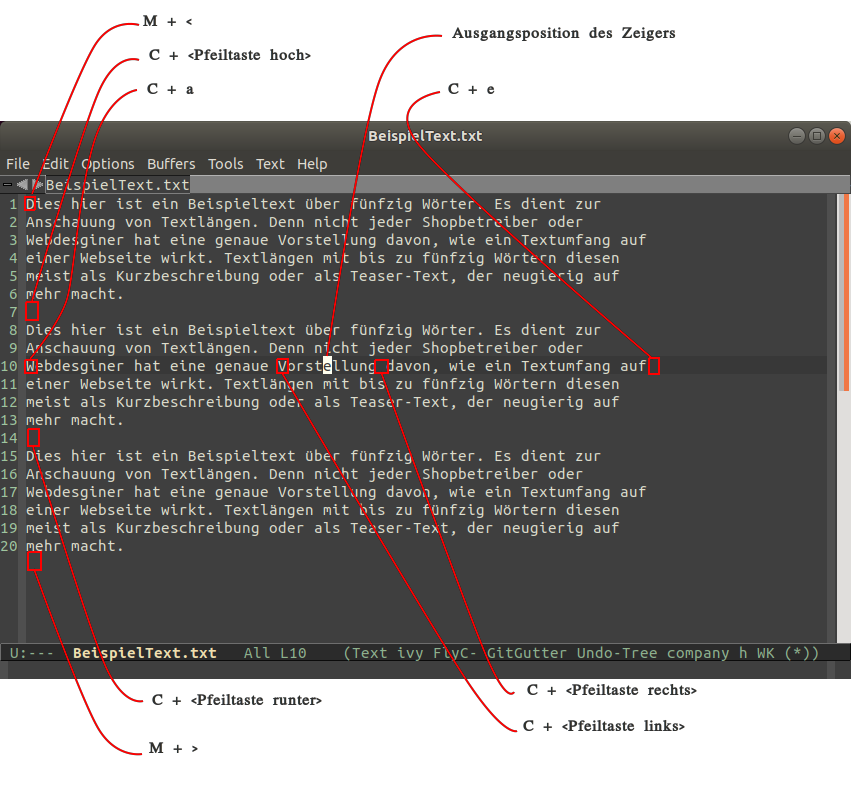
\includegraphics[width=.95\textwidth]{./images/Grundlagen/Navigation.png}
  \caption{\label{fig:Navigation} Diese Abbildung veranschaulicht die
    Sprünge des Zeigers mit unterschiedlichen Tastenkombinationen.}
\end{figure}
Um den sichtbaren Bereich des Textes zu verschieben, werden folgende
Tastenkombinationen verwendet:

\begin{itemize}
\item \textbf{C-v}: Seite nach oben {\glqq}verschieben{\grqq}.
\item \textbf{M-v}: Seite nach unten {\glqq}verschieben{\grqq}.
\item \textbf{C-l}: Mittiges Ausrichten der Seite bezogen auf die
  Position des Zeigers. Erneutes ausführen der Tastenkombination
  verschiebt die Zeile in der sich der Zeiger befindet an den oberen
  Rand des Bildschirms, danach an den unteren Rand und danach wieder
  in die Mitte.\\
\end{itemize}
Es gibt einige weitere Möglichkeiten um in Emacs zu navigieren. Dafür
stehen bereits eine Vielzahl an Tutorials zur Verfügung. Ein solches
ist das in Emacs enthaltene Tutorial. Dieses kann direkt in Emacs mit
der Tastenkombination \textbf{C-h t} aufgerufen
werden. \cite{CameronRosenblattRaymond1996}\\

\section{Hilfe}
Emacs hat eine eingebaute Hilfe. Die Tastenkombination für die Hilfe
ist: \textbf{C-h} gefolgt von einem weiteren Buchstaben. Mit der
Tastenkombination \textbf{C-h ?} wird die Hilfe für die Hilfe
aufgerufen. Hier wird alles über die Verwendung der Hilfe
erklärt. Beendet wird die Hilfe mittels
\textbf{C-g}. \cite{CameronRosenblattRaymond1996}\\\\ Weitere
hilfreiche Tastenkombinationen für die Hilfe sind:
\begin{itemize}
\item \textbf{C-h c}: Gibt den Namen der Funktion im
  \textit{minibuffer} (siehe Abschnitt \ref{sec:emacsstart}) aus,
  welche für die eingetippte Tastenkombination ausgeführt wird.
\item \textbf{C-h k}: Beschreibt die Funktion, die hinter der
  eingetippten Tastenkombination steckt.
\item \textbf{C-h f}: Beschreibt die eingetippte Funktion.
\item \textbf{C-h v}: Beschreibt die eingetippte Variable.\\
\end{itemize}

\section{Puffer}
\label{sec:puff}
Wird in Emacs ein Text editiert, so geschieht dies in Emacs in einem
Puffer. Wenn eine Datei geöffnet wird, dann wird der Text von Emacs in
einem Puffer gehalten. Beim Start von Emacs wird immer ein Puffer
namens \textit{*scratch*} erstellt. Hinter diesem Puffer befindet sich
keine Datei. Soll der Inhalt des Puffers dennoch abgespeichert werden,
so muss ein Dateiname angegeben werden. \cite{PufferInEmacs}\\\\ Die
wichtigsten Tastenkombinationen für Puffer sind:
\begin{itemize}
\item \textbf{C-x b}: Damit kann zwischen offenen Puffern gewechselt
  werden. Ist kein Puffer mit dem eingegebenem Namen verfügbar, so
  wird ein neuer Puffer angelegt.
\item \textbf{C-x C-b}: Dieser Befehl öffnet eine Liste mit allen
  offenen Puffern. In der {\glqq}Pufferliste{\grqq} können alle
  offenen Puffer verwaltet werden.\\
\end{itemize}

\section{Modi}
Emacs verhält sich beim Editieren unterschiedlich, je nachdem welche
Modi aktiv sind. Es gibt zwei Arten von Modi, die \textit{major modes}
und die \textit{minor modes}. Für jeden Puffer kann immer nur ein
\textit{major mode} zur selben Zeit aktiv sein. Jedoch kann ein Puffer
immer über beliebig viele \textit{minor modes} verfügen. \cite{EmacsManual}\\

\subsection{Major Modes}
\label{subsec:majormodes}
\textit{Major modes} legen fest, nach welchen grundlegenden Regeln der
Text in einem Puffer editiert wird. Das kann ein Text-Dokument sein,
welches den \textit{text-mode} verwendet. Zum Programmieren hingegen,
werden eigene Modi zur Verfügung gestellt. Ein Beispiel für C++-Code
ist der \textit{c++-mode}. Emacs wählt den \textit{major mode} anhand
der Dateiendung. \cite{EmacsManual}\\

\subsection{Minor Modes}
Ein Puffer kann beliebig viele \textit{minor modes} zur gleichen Zeit
verwenden. Diese fügen weitere Funktionalität zum Editieren hinzu,
ohne dass der \textit{major mode} verändern werden muss. Ein
\textit{minor mode} ist zum Beispiel der
\textit{flyspell-mode}. Dieser führt eine Prüfung der Rechtschreibung
während des Schreibens durch. Werden Pakete (siehe Abschnitt
\ref{sec:paketebasics}) zu Emacs hinzugefügt, so enthalten diese oft
auch einen \textit{minor mode}. \cite{EmacsManual}\\

\section{Fenster und Rahmen}
In Emacs gibt es Fenster (\textit{windows}) und Rahmen
(\textit{frames}). Es ist zu beachten, dass ein Unterschied zwischen
einem \textit{window} in Emacs und einem \textit{window} in
\textit{win10} besteht. \textit{Frames} können mit \textit{windows} in
\textit{win10} verglichen werden. Diese sind eigenständige Rahmen, in
denen sich ein oder mehrere Fenster befinden können. Dies ist nützlich
wenn zum Beispiel mehrere Bildschirme verwendet werden und auf diesen
Bildschirmen die selbe Instanz von Emacs laufen soll. \textit{Windows}
sind Fenster innerhalb eines Rahmens. In diesen Fenstern sind die
Puffer direkt geöffnet. So kann ein Rahmen in mehrere Fenster
unterteilt werden. In unterschiedlichen Fenstern kann auch der selbe
Puffer geöffnet sein. \cite{EmacsManual}\\\\ Die wichtigsten
Tastenkombinationen zum verwalten von \textit{windows} und
\textit{frames} sind:
\begin{itemize}
\item \textbf{C-x 2}: Spaltet das aktuelle \textit{window} in zwei
  \textit{windows} untereinander.
\item \textbf{C-x 3}: Spaltet das aktuelle \textit{window} in zwei
  \textit{windows} nebeneinander.
\item \textbf{C-x 0}: Schließt das aktuelle \textit{window}.
\item \textbf{C-x 1}: Maximiert das aktuelle \textit{window} auf die
  Große des \textit{frames}.
\item \textbf{C-x 5 2}: Erzeugt ein weiteres \textit{frame}.
\item \textbf{C-x 5 0}: Schließt das aktuelle \textit{frame}.
\item \textbf{C-x o}: Damit kann zwischen den \textit{windows} im
  aktuellen \textit{frame} gewechselt werden.\\
\end{itemize}

\section{Emacs starten}
\label{sec:emacsstart}
Emacs wird am einfachsten gestartet, in dem \textit{emacs} in die
Konsole getippt wird. Es können natürlich auch Verknüpfungen verwendet
werden. Wird \textit{emacs} gefolgt von einem Dateinamen eingetippt,
wie zum Beispiel \texttt{emacs testdatei}, so wird die Datei
{\glqq}testdatei{\grqq} mit emacs geöffnet. Diese Datei kann eine
beliebige oder auch gar keine Endung haben. Existiert die Datei noch
nicht, so öffnet Emacs einen Puffer mit diesem angegebenen Namen. Erst
wenn der Puffer gespeichert wird (\textbf{C-x C-s}), legt Emacs eine
Datei mit dem angegebenen Namen an.

Innerhalb von Emacs wird eine Datei mit der Tastenkombination
\textbf{C-x C-f} geöffnet. Existiert diese Datei nicht, so wird
ebenfalls nur ein Puffer mit dem Namen angelegt und erst beim
Abspeichern die Datei erstellt.

Wurde aus Versehen eine falsche Tastenkombination eingegeben, kann der
Befehl mit \textbf{C-g} abgebrochen werden. Eine weiter Möglichkeit
ist es drei mal die esc-Taste zu drücken (\textbf{<esc> <esc> <esc>}).

Jeder Befehl in Emacs ist ein Funktionsaufruf, welcher in der Sprache
Emacs Lisp geschrieben ist. Diese Funktionen können auch direkt
aufgerufen werden. Eine Möglichkeit ist die Tastenkombination
\textbf{M-x}, welche den Zeiger in den \textit{minibuffer} springen
lässt. Dort kann die gewünschte Funktion eingetippt werden.

Beendet wird Emacs mit der Tastenkombination \textbf{C-x C-c}. Sind
Puffer offen, welche noch nicht abgespeichert wurden. So wird der/die
Benutzer/in darauf aufmerksam gemacht, bevor Emacs beendet wird
\cite{Hahn2016, CameronRosenblattRaymond1996}.

In der Grafik \ref{fig:Emacsscr} ist ein Fenster von Emacs zu sehen.
Dieses Fenster wird beim Start von Emacs, ohne Konfigurationen
angezeigt. Ganz oben befindet sich die Menüleiste. Diese Leiste kann
nützlich sein, wenn Tastenkombinationen für einzelne Befehle vergessen
wurden. Denn in den Tabs der Menüleiste sind neben dem Kommando auch
die Tastenkombinationen zu sehen. Ein Mausklick auf den Tab
\textit{File} öffnet diesen und neben \textit{Save} steht die
Tastenkombination \textbf{C-x C-s}.

Direkt unter der Menüleiste befindet sich im Grunde die
Symbolleiste. Hier befinden sich Verknüpfungen zu häufig verwendeten
Kommandos. Diese Leiste ist in Emacs überflüssig, weil für jede
Verknüpfung eine Tastenkombination vorhanden ist. Unterhalb befindet
sich der geöffnete Puffer mit dem Zeiger. Unter dem Puffer befindet
sich die sogenannte {\glqq}\textit{mode line}{\grqq}. In der
\textit{mode line} stehen einige Informationen über den Puffer und den
Zeiger. Das erste was auf der \textit{mode line} zu sehen ist (links),
ist der Name des Puffers. Danach folgt eine prozentuale Anzeige. Kann
der gesamte Puffer angezeigt werden, so steht dort
{\glqq}\textit{All}{\grqq}, wie auch in der Grafik. Ist der Puffer zu
groß für das Fenster, so wird eine Prozentzahl angezeigt wo im Puffer
man sich gerade befindet. Befindet man sich in der Mitte des Puffers,
so wird 50 \% angezeigt. Eine Ausnahme sind der Anfang und das Ende
des Puffers, dort wird {\glqq}\textit{Top}{\grqq} beziehungsweise
{\glqq}\textit{Bot}{\grqq} angezeigt. An der nächsten Stelle steht, in
welcher Zeile sich der Zeiger befindet. In der Grafik befindet sich
der Zeiger in der vierten Zeile. Danach folgt in Klammern die Angabe
der Modi. Ein Puffer kann sich in einem \textit{major mode} und
beliebig vielen \textit{minor modes} befinden. Im Beispiel ist
{\glqq}\textit{Lisp}{\grqq} der \textit{major mode} und
{\glqq}\textit{Interaction}{\grqq} der \textit{minor mode}. Unter der
\textit{mode line} befindet sich noch der \textit{minibuffer}. Im
\textit{minibuffer} werden eingetippte Tastenkombinationen
wiedergegeben. Wenn eine Tastenkombination zusätzliche Eingabe
erfordert wird diese ebenfalls dort eingegeben.\\

\begin{figure}[h]
  \centering
  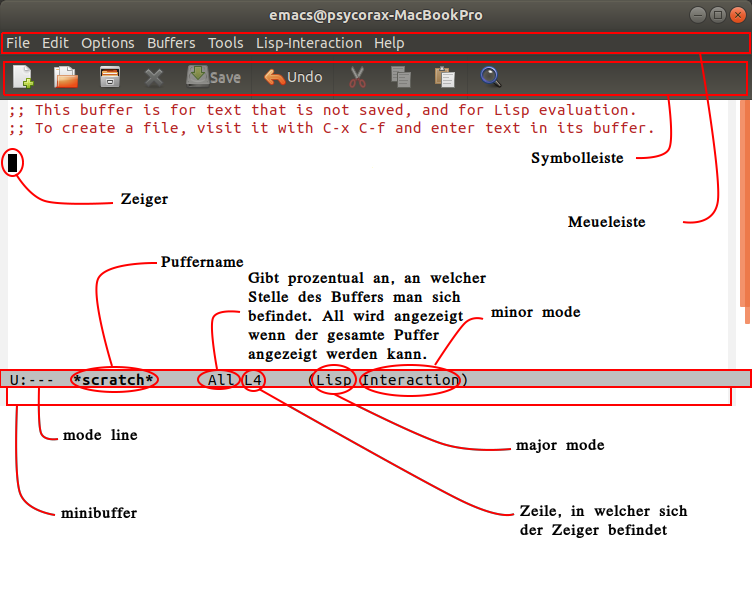
\includegraphics[width=.95\textwidth]{./images/Grundlagen/Emacsscreen.png}
  \caption{\label{fig:Emacsscr} Ein Emacs-Rahmen mit einem Fenster in
    der \textit{Default}-Konfiguration.}
\end{figure}

\section{Die Konfigurationsdatei}
\label{sec:konfdatgl}
Emacs kann an die persönlichen Anforderungen angepasst werden. Um
diese Anpassungen nicht für jede Sitzung neu vornehmen zu müssen,
geschieht dies in Form einer Konfigurationsdatei. Diese Datei wird bei
jedem Start von Emacs geladen. Ist keine Konfigurationsdatei
vorhanden, so startet Emacs mit den Standardeinstellungen. Emacs sucht
drei verschiedene Konfigurationsdateien unter \cite{EmacsInitfile}:
\begin{itemize}
\item $\sim$/.emacs
\item $\sim$/.emacs.d
\item $\sim$/.emacs.d/init.el
\end{itemize}
Das Tilde-Symbol {\glqq}$\sim${\grqq} kennzeichnet das
\textit{Home}-Verzeichnis.  Wenn eine dieser drei Dateien gefunden
wird, so wird diese zur Initialisierung verwendet. In dieser Arbeit
wird zur Konfiguration die Datei \textit{init.el} im Verzeichnis
\textit{$\sim$/.emacs.d/} verwendet.

In dieser Datei, können beliebig viele Konfigurationen vorgenommen
werden. Da sich Emacs nur anhand dieser Datei konfiguriert, kann auf
jedem Gerät Emacs mit den selben Einstellungen gestartet werden. Diese
Konfigurationen sind in der Programmiersprache \textit{Emacs Lisp}
(siehe Abschnitt \ref{sec:emacslisp}) geschrieben, was auch die Endung
{\glqq}el{\grqq} verrät.

Mögliche Konfigurationen sind:
\begin{itemize}
\item Anpassen der Tastenkombinationen an die eigenen Bedürfnisse,
\item Einstellungen, welche Modi wann aktiv sein sollen und generelle
  Konfigurationen an Modi,
\item Einstellen beliebiger Farbschemata und generell der
  Benutzeroberfläche,
\item Installieren zusätzlicher Pakete und
\item Definieren eigener Funktionen.\\
\end{itemize}
Der Aufbau der Konfiguration wie sie in dieser Arbeit durchgeführt
wird, ist nicht nur auf eine Datei beschränkt. Es können in der
verwendeten Datei \textit{init.el} weitere Dateien geladen
werden. Diese sind \textit{org}-Dateien. Durch die Auslagerung der
Konfigurationen auf diese \textit{org}-Dateien wird die Konfiguration
übersichtlicher.\\

\section{Pakete}
\label{sec:paketebasics}
Pakete sind Erweiterungen, welche zusätzliche Funktionalität für Emacs
implementieren. Es gibt Pakete, die standardmäßig installiert
sind. Diese sind in dem Archiv {\glqq}GNU{\grqq} vorhanden. Zusätzlich
zu diesen gibt es Pakete von der \textit{Community}. Das größte Archiv
in dem diese Pakete gesammelt werden ist
\textit{melpa}\footnote{\url{https://melpa.org/}}. Emacs bietet
einfache Möglichkeiten um Pakete zu installieren. Die Installation
kann direkt im \textit{minibuffer} erfolgen. Der Nachteil an dieser
Methode ist, dass bei einer Neuinstallation von Emacs diese Pakete
nicht mehr vorhanden sind. Eine Abhilfe schafft der Installationsweg
über eine Konfigurationsdatei. In dieser können alle beliebigen Pakete
angegeben werden, welche von Emacs beim Start geladen werden
sollen. Die verfügbaren Pakete können mittels \textbf{M-x
  package-list-packages} angezeigt werden. \\

\section{Emacs Lisp}
\label{sec:emacslisp}
Die Programmiersprache \textit{Emacs Lisp} ist ein Dialekt der
Programmiersprache \textit{Lisp}. \textit{Emacs} selbst ist zum
größten Teil in dieser Sprache programmiert. Aus diesem Grund werden
auch die Erweiterungen in dieser Sprache geschrieben. \textit{Emacs
  Lisp} arbeitet mit Listen und Listen von Listen. In \textit{Lisp}
wird alles in Form von Listen verarbeitet und abgespeichert. Das
bedeutet, Daten und Programme werden auf die gleiche Art
repräsentiert. Dadurch ist es sehr einfach ein Programm als ein Datum
für ein anderes Programm zu verwenden. Eine Liste wird definiert, in
dem alle Elemente der Liste zwischen Klammern geschrieben werden, die
einzelnen Elemente werden durch Leerzeichen getrennt. \cite{EmacsLisp}

Ein einfache Liste ist: {\glqq}(+ 2 3){\grqq}. Diese Liste besteht nun
aus einem Plus-Symbol, einer eins und einer zwei. Das erste Symbol der
Liste wird von dem System als Kommando interpretiert. Das Plus-Symbol
ruft ein Funktion zum Addieren auf. Diese Funktion lässt beliebig
viele Parameter zu. In diesem Fall sind es zwei Parameter. Die Liste
kann mit \textbf{C-x C-e} ausgeführt werden. Im \textit{minibuffer}
wird das Ergebnis {\glqq}5{\grqq} angezeigt. Sollte vor der Liste ein
Hochkomma {\glqq}'{\grqq} stehen, so wird beim Ausführen der Liste
nach keinem Kommando an erster Stelle gesucht. Derselbe Effekt wird
mit dem Begriff {\glqq}quote{\grqq} erzielt. Es wird die Liste einfach
so wie sie ist ausgegeben. Als Beispiel wird die Liste '(+ 2 3)
verwendet, welche dasselbe aussagt wie (quote(+ 2 3)). Nach Ausführen
der Liste wird im \textit{minibuffer} die Liste (+ 2 3) ausgegeben, da
das erste Element der Liste nicht als Kommando interpretiert wird. In
der angeführten Grafik \ref{fig:elisp}, sind beide Listen zu
sehen. Diese Listen wurden mit der Tastenkombination \textbf{C-j}
ausgeführt. Der Unterschied zwischen \textbf{C-x C-e} und \textbf{C-j}
ist, dass bei \textbf{C-j} das Ergebnis zusätzlich in den Puffer
geschrieben wird.\\

\begin{figure}[h]
  \centering
  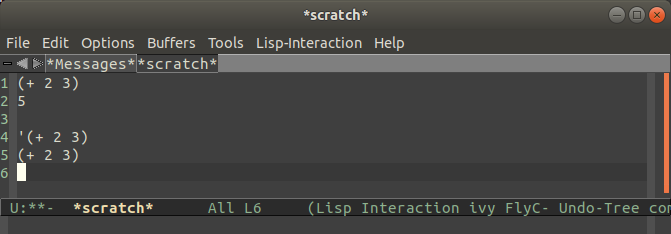
\includegraphics[width=.95\textwidth]{./images/Grundlagen/Elisp.png}
  \caption{\label{fig:elisp}Zweimal der selbe Inhalt in einer
    Liste. Einmal wurde die Liste mit voranstehendem Hochkomma und
    einmal ohne ausgeführt.}
\end{figure}

\section{Der Modus org}
\label{sec:orgmode}
Der \textit{org-mode} ist ein \textit{major-mode} in Emacs. Der Modus
dient zur Verarbeitung von Text und wird für folgende Aufgaben
verwendet:
\begin{itemize}
\item Zum Niederschreiben von Notizen,
\item Für das Erstellen von \textit{TODO-Listen} und
\item Zur Planung von Projekten.
\end{itemize}
Der \textit{org-mode} wird ebenfalls dazu verwendet, um
Programmiersprachen einfach und leserlich für Menschen
darzustellen. Der Modus ist ein einfach in der Verwendung und gut
geeignet für Einsteiger. Wird mehr Funktionalität benötigt, steht
diese ebenfalls zur Verfügung. \cite{OrgMode}

\textit{Org-mode} ist in Emacs standardmäßig enthalten, es kann jedoch
eine aktuellere Version installiert werden. Der Modus wird automatisch
verwendet, wenn eine Datei mit der Endung {\glqq}.org{\grqq} in einen
Puffer geladen wird. Der \textit{org-mode} kann auch manuell mit dem
Kommando \texttt{M-x org-mode} aktiviert werden.\\

\subsection{Die Installation von org-mode}
In dieser Arbeit wird die Version
\textit{org-elpa}\footnote{\url{https://orgmode.org/elpa.html}}
installiert. Es muss darauf geachtet werden, dass vor der Installation
in der Konfigurationsdatei keine \textit{org}-Funktion ausgeführt
wird. Aus diesem Grund erfolgt die Installation in der Datei
{\glqq}init.el{\grqq}, noch vor dem Laden der \textit{org}-Datei. Der
Grund warum \textit{org-mode} aktualisiert wird ist, dass die aktuelle
Version Text-Hervorhebung für \textit{org} Dateien innerhalb von
Code-Blöcken ermöglicht.\\

\subsection{Kapitel und Überschriften}
\label{subsec:kapitel}
\textit{Org} kann so wie \textit{Latex} mit Kapitel und
       {\glqq}Unterkapitel{\grqq} organisiert werden. Die Überschrift
       eines Kapitels beginnt mit einem Stern, gefolgt von einem
       Leerzeichen. Die Überschrift eines Unterkapitels hat zwei
       Sterne gefolgt von einem Leerzeichen, dies setzt sich so
       fort. Damit können {\glqq}Bäume{\grqq} aufgebaut werden. Unter
       diesen Überschriften kann jeder beliebige Inhalt stehen. Die
       Funktion \texttt{org-cycle} ist auf die Taste \textbf{TAB}
       gebunden, damit können die einzelnen Inhalte der Überschriften
       ein und ausgeblendet werden. Es gibt drei Zustände:
\begin{itemize}
\item \textbf{folded} : Alles bis auf die Überschriften der Kapitel
  ist sichtbar.
\item \textbf{children} : Alle Überschriften sind sichtbar.
\item \textbf{subtree} : Alle Überschriften und Inhalte sind sichtbar.
\end{itemize}
Ist der Inhalt einer Überschrift ausgeblendet, so wird dies durch drei
Punkte am Ende der Überschrift gekennzeichnet. Es gibt die Funktion
\texttt{org-global-cycle}. Diese ist auf die Tastenkombination
\textbf{<shift> TAB} gebunden. Diese besitzt ebenfalls drei
Zustände. Der Unterschied zu der Funktion \texttt{org-cycle} ist, dass
sie für alle Überschriften in der Datei gelten. Die Namen der Zustände
sind:
\begin{itemize}
\item \textit{OVERVIEW}
\item \textit{CONTENTS}
\item \textit{SHOW ALL}
\end{itemize}
Mit der Hilfe dieser Funktionalität von \textit{org} ist es einfacher,
den Überblick über große Dateien zu bewahren. In der folgenden Grafik
\ref{fig:headlines} sind dreimal die selben Kapitel mit der selben
Anzahl an Unterkapitel und selbem Inhalt in unterschiedlichen
Zuständen dargestellt. Es sind am Ende einiger Überschriften die drei
Punkte zu erkennen. Das Inhalt versteckt ist, ist auch den
Zeilennummern zu entnehmen.\\

\begin{figure}[h]
  \centering
  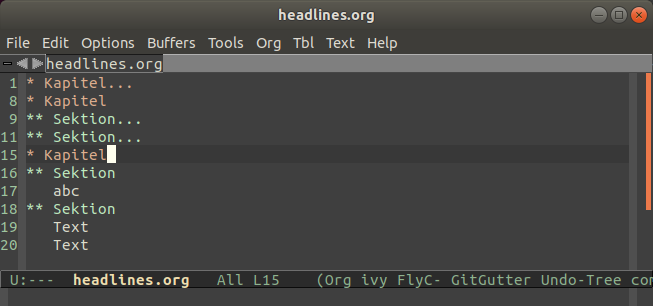
\includegraphics[width=.95\textwidth]{./images/KonfigurationUndPakete/headlines.png}
  \caption{\label{fig:headlines} Das erste Kapitel hat den Zustand
    {\glqq}folded{\grqq}. Das zweite Kapitel hat den Zustand
    {\glqq}children{\grqq}. Das dritte Kapitel hat den Zustand
    {\glqq}subtree{\grqq}.}
\end{figure}

Eine weitere Funktionalität ist, dass diese Kapitel und Unterkapitel
verschoben werden können. Dies kann mit den Pfeil-Tasten bei
gedrückter alt-Taste durchgeführt werden. Dazu muss sich der Zeiger
auf der zu verschiebenden Überschrift befinden. Die Reihenfolge der
Kapitel und Unterkapitel kann dadurch einfach verändert werden. Es
können Unterkapitel in andere Kapitel verschoben werden. Außerdem kann
auch ein Unterkapitel in der Hierarchie nach {\glqq}außen{\grqq}
geschoben werden, wodurch aus diesem Unterkapitel ganz einfach ein
eigenständiges Kapitel wird. Dadurch wird das Umstrukturieren der
Datei sehr einfach.

Es ist möglich, die Überschriften mit einem {\glqq}TODO{\grqq} oder
{\glqq}DONE{\grqq} zu versehen. Dies kann mit den Pfeil-Tasten bei
gehaltener shift-Taste durchgeführt werden. Dazu muss sich der Zeiger
auf einer Überschrift befindet.\\

\subsection{Makros}
\label{subsec:makro}
Beim Öffnen einer \textit{org}-Datei wird diese standardmäßig im
Zustand \textit{OVERVIEW} gezeigt. Ist dies nicht erwünscht, kann am
Anfang der Datei ein beliebiger Zustand mit Hilfe des Makros
\textit{\#+STARTUP} gesetzt werden. Die Möglichkeiten sind:
\begin{itemize}
\item \texttt{\#+STARTUP: overview}
\item \texttt{\#+STARTUP: content}
\item \texttt{\#+STARTUP: showall}
\item \texttt{\#+STARTUP: showeverything}
\end{itemize}
Der Zustand \textit{showeverything} zeigt zusätzlich auch die
versteckten Teile der Datei an. Die anderen Zustände wurden in
Abschnitt \ref{subsec:kapitel} bereits beschrieben.

Es gibt noch weitere vordefinierte Makros für den \textit{org-mode}
welche beim Exportieren von Dateien nützlich sind. Am häufigsten in
Verwendung sind:
\begin{itemize}
\item \textbf{\#+AUTHOR} : Der Name des Autors
\item \textbf{\#+DATE} : Datum
\item \textbf{\#+TITLE} : Titel der Datei
\item \textbf{\#+CAPTION} : Kurzbeschreibung
\end{itemize}

\subsection{Codeblöcke}
In \textit{org} können Codeblöcke eingefügt werden. Dies geschieht in
Form eines Makros (siehe Abschnitt \ref{subsec:makro}). Vor dem
Quellcode steht \texttt{\#+BEGIN\_SRC} und nach dem Quellcode steht
\texttt{\#+END\_SRC}. Alles was innerhalb dieser beiden Makros steht,
wird als Quellcode interpretiert. In der selben Zeile nach dem Makro
{\glqq}\texttt{\#+BEGIN\_SRC}{\grqq} kann einen Programmiersprache
definiert werden. Dadurch weiß Emacs welcher \textit{major-mode} zu
verwenden ist. Dies wird benötigt, damit die Formatierung und
Hervorhebung des Textes korrekt dargestellt werden kann. Der Codeblock
kann in \textit{org-mode} direkt mit der Tastenkombination \textbf{C-c
  C-c} evaluiert werden. Nach Ausführen des Codeblocks wird
automatisch das Makro \textit{\#+RESULT} erzeugt. Unterhalb dieses
Makros wird der Rückgabewert angegeben. Beispiele für einen
ausgeführten Emacs Lisp-Codeblock und einen Python-Codeblock folgen.\\

\lstinputlisting[language=Lisp, firstline=1,
  lastline=17]{./code/Pakete/Codeblock.org}

Codeblöcke mit Latex-Code sind sehr nützlich, wenn die Datei mittels
Latex exportiert wird (siehe Abschnitt \ref{subsec:export}). Dadurch
können Bilder, Tabellen oder mathematische Formeln wie gewohnt in
{\glqq}Latex{\grqq} geschrieben werden.\\

\subsection{Exportieren}
\label{subsec:export}
\textit{Org} kann Text in verschiedene {\glqq}Formate{\grqq}
exportieren. Die wichtigsten sind:
\begin{itemize}
\item Latex
\item PDF
\item HTML
\end{itemize}
Wenn eine PDF-Datei erzeugt werden soll, kann diese mittels Latex
exportiert werden. Das bedeutet, dass aus der \textit{org}-Datei eine
\textit{tex}-Datei erzeugt wird und diese dann zum Erzeugen einer
\textit{PDF-Datei} verwendet wird. \textit{Org}-Dateien können auch in
eine \textit{HTML}-Datei exportiert werden. Dadurch lassen sich
einfache Webseiten realisieren. Diese \textit{HTML}-Dateien eigenen
sich auch als einfache Präsentationen.\\

\subsection{Tabellen}
In \textit{org} können sehr einfach Tabellen erstellt werden. Spalten
werden mittels {\glqq}|{\grqq} unterteilt. Die oberste Reihe der
Tabelle gibt die Anzahl der Spalten vor. Darunter wird einfach
{\glqq}|-{\grqq} und die Tabulator-Taste gedrückt. Ein Beispiel einer
solchen Tabelle:\\

\lstinputlisting[language=Lisp, firstline=1,
  lastline=3]{./code/Pakete/Tabellen.org}

Nach dem Eintragen der Daten, passt die Tabelle automatisch die Größe
der Spalten und Zeilen an. Die Tabelle kann mit der Tastenkombination
\textbf{C-c C-c} manuell ausgerichtet werden. Die Spalten und Zeilen
können mit den Pfeiltasten bei gedrückter ALT-Taste vertauscht
werden. Die Tastenkombination \textbf{C-c \^} sortiert die Inhalte
einer Tabelle. In der folgenden Tabelle sind die Einträge alphabetisch
sortiert. Es ist ebenfalls erkennbar, dass sich die Spaltenbreite an
die längste Zeichenkette der Spalte angepasst hat.\\

\lstinputlisting[language=Lisp, firstline=4,
  lastline=10]{./code/Pakete/Tabellen.org}

\chapter{Pakete}
\label{cha:pakete}
Hier werden alle verwendeten Pakete beschrieben. Diese Beschreibung
umfasst die Funktionalität und die verwendete Konfiguration der
Pakete.\\

\section{Grundlagen für die Konfiguration der Pakete}
\label{sec:basicsKonfig}
Es folgt eine Beschreibung des Paketes \textit{use-package}. Dieses
Paket wird zum Installieren und Konfigurieren aller weiteren Pakete
verwendet. Im Anschluss werden noch einige Funktionen der Sprache
Emacs Lisp beschrieben. Diese Funktionen werden für die Definition
eigener Funktionen benötigt.\\

\subsection{Use-Package}
\label{subsec:usepackage}
Das Paket \textit{use-package} verwendet die Emacs Lisp-Funktion
\textit{require}. Die Funktion \textit{require} ist in Emacs
standardmäßig implementiert. Sie erwartet einen Parameter, den Namen
eines Paketes. Die Funktion überprüft ob ein Paket mit dem Namen
bereits installiert ist. Ist dies nicht der Fall, wird das Paket
installiert. Durch die Verwendung des Paketes \textit{use-package}
wird eine einfachere Installation und Konfiguration von Paketen
ermöglicht.

Um ein gewünschtes Paket zu installieren wird erst das Kommando
{\glqq}use-package{\grqq} geschrieben, gefolgt von dem Namen des
Pakets. In dem folgendem Beispiel \ref{code:usepack}, wird das Paket
\textit{example-pack} verwendet. Es gibt einige Schlüsselwörter für
\textit{use-package}, alle beginnen mit einem
Doppelpunkt. \cite{UsePackage}\\\\ Die am häufigsten verwendeten
Schlüsselwörter folgen:
\begin{itemize}
\item \textbf{:ensure}: Folgt auf dieses Schlüsselwort der Parameter
  {\glqq}t{\grqq} für \textit{true}, so wird das Paket installiert. Es
  ist ebenfalls möglich, die Variable
  \textit{use-package-always-ensure} auf {\glqq}t{\grqq} zu setzen,
  dann wird das Verhalten von {\glqq}\textit{:ensure} t{\grqq} global
  auf alle Pakete angewendet.
\item \textbf{:init}: Nach diesem Schlüsselwort kann beliebig viel
  Emacs Lisp-Code stehen. Zu beachten ist, dass dieser Code
  \textbf{vor} dem Laden des Paketes abgearbeitet wird.
\item \textbf{:config}: Funktioniert gleich wie \textit{:init}, nur
  das dieser Code \textbf{nach} dem Laden des Paketes abgearbeitet
  wird.
\item \textbf{:bind}: Wird dazu verwendet um Tastenkombinationen
  spezifisch für dieses Paket festzulegen. Die Syntax lautet
  folgendermaßen: Erst die Tastenkombination unter doppelten
  Hochkomma, danach ein Punkt und darauf die gewünschte
  Funktionalität, mit der die Tastenkombination verknüpft
  wird. Codestück \ref{code:usepack} in Zeile fünf veranschaulicht
  dies.
\item \textbf{:map}: Dies ist eine Erweiterung für \textit{:bind}, um
  Tastenkombinationen spezifisch für einzelne Modi festlegen zu
  können. Die Syntax ist gleich wie bei \textit{:bind}, nur dass vor
  der Tastenkombination mit \textit{:map} der Modus festgelegt wird.
\item \textbf{:pin}: Mit \textit{:pin} kann direkt ausgewählt werden,
  von welchem Archiv das Paket geladen werden soll.
\item \textbf{:hook}: Dieses Schlüsselwort dient dazu, \textit{minor
  modes} an andere Modi anzuhängen. Im folgenden Beispiel wird der
  \textit{b-mode} an den \textit{a-mode} angehängt. Das bedeutet, wird
  \textit{a-mode} verwendet, so wird automatisch auch \textit{b-mode}
  aktiviert.
\item \textbf{:after}: Mit \textit{:after} kann festgelegt werden,
  welche Pakete installiert und geladen sein müssen, bevor dieses
  Paket geladen wird. Dadurch wird eine Reihenfolge für das Laden der
  Pakete definiert. Dies ist manchmal notwendig, da einige Pakete auf
  anderen aufbauen und dadurch selbstständig nicht korrekt geladen
  werden. In dieser Liste kann eine beliebige Anzahl an Paketen
  stehen.
\item \textbf{:custom}: Das Schlüsselwort \textit{:custom} wird
  verwendet, um Variable mit einem Wert zu belegen. Die Syntax lautet
  folgendermaßen: Erst der Name der Variable, danach folgt der Wert
  der zugewiesen wird, gefolgt von einem Kommentar. Codestück
  \ref{code:usepack} in Zeile neun veranschaulicht dies.
\end{itemize}

\begin{program}[h]
  \lstinputlisting[language=Lisp, firstline=1,
    lastline=10]{./code/Pakete/usepackage.el}
  \caption{\label{code:usepack}Dieses Codestück zeigt die Verwendung
    des Pakets \textit{use-package} mit {\glqq}Dummy{\grqq}-Werten.}
\end{program}

\subsection{Kommandos für die Konfiguration}
\label{subsec:kommandosKonfig}
Hier werden einige Emacs Lisp-Kommandos und Code-Zeilen aufgelistet,
welche in den Konfigurationsdateien verwendet werden:
\begin{itemize}
\item \textit{setq} : Definiert eine Variable global mit einem Wert.
\item \textit{add-hook} : Bindet zwei Objekte aneinander. Diese
  Objekte können Modi, Funktionen oder Tastenkombinationen sein.
\item \textit{defun} : Definiert eine Funktion.
\item \textit{unless} : Funktioniert wie ein if-Statement, jedoch wird
  der Code darunter ausgeführt wenn das Statement falsch
  {\glqq}nil{\grqq} ist.
\item \textit{progn} : Ermöglicht es, mehrere Funktionen
  hintereinander abzuarbeiten.
\item \textit{message} : Schreibt eine Zeichenkette in den
  {\glqq}message{\grqq} Puffer.
\item \textit{concat} : Fügt eine Zeichenkette aus mehreren kleinen
  Zeichenketten zusammen.
\item \textit{shell-command} : Führt ein Kommando in der Konsole aus.
\item \textit{file-exists-p} : Überprüft, ob eine Datei mit dem
  angegebenen Namen existiert.
\item \textit{file-directory-p} : Überprüft, ob ein Ordner mit dem
  angegebenen Namen existiert.
\item \textit{cd} : Wechselt das Verzeichnis.
\item \textit{find-file} : Öffnet eine Datei mit dem angegebenen
  Namen.
\item \textit{mkdir} : Erzeugt einen Ordner.
\end{itemize}

\section{Pakete zur Navigation}
\label{sec:navigation}
Die folgenden Pakete vereinfachen die Navigation in Emacs. Diese
vereinfachte Navigation erfolgt mit der Hilfe von Suchfunktionen
innerhalb eines Puffers. Es folgen ebenfalls Pakete für die
automatische Vervollständigung im \textit{minibuffer}.

\subsection{Avy}
\label{subsec:avy}
Das Paket \textit{Avy} wird verwendet, um an jede beliebige Position
im sichtbaren Bereich zu springen. Dies funktioniert über mehrere
Fenster, jedoch nur innerhalb eines Rahmens. \textit{Avy} stellt
folgende Funktionen zur Verfügung: \textit{avy-goto-char} und
\textit{avy-goto-char-2}. Wird die Funktionen \textit{avy-goto-char}
aufgerufen gefolgt von einem Zeichen zu dem gesprungen werden soll,
dann sucht \textit{avy} nach allen Stellen im sichtbaren Bereich, die
mit diesem Zeichen übereinstimmen. Alle Übereinstimmungen werden mit
Buchstaben markiert und durch Eintippen dieser Buchstaben springt der
Zeiger zu der gewünschten Position. Die Funktion
\textit{avy-goto-char-2} funktioniert identisch, nur dass diese
Funktion zwei Parameter nimmt, dadurch sind die Übereinstimmungen
geringer. Die folgende Grafik \ref{fig:avy} veranschaulicht diese
Beschreibung. In der Abbildung wird dieser Text zur Beschreibung des
Paketes \textit{avy} angezeigt.  Zum Springen wird die Funktion
\textit{avy-goto-char-2} verwendet. Gesprungen werden soll zu dem
vorletzten {\glqq}Avy{\grqq} im angezeigtem Fenster. In der Abbildung
sind alle {\glqq}av{\grqq} mit Buchstaben markiert. Um zu dem
gewünschten Zeichen zu springen müssen die Buchstaben {\glqq}l{\grqq}
und {\glqq}h{\grqq} eingetippt werden. \cite{Avy}

\begin{figure}[h]
  \centering
  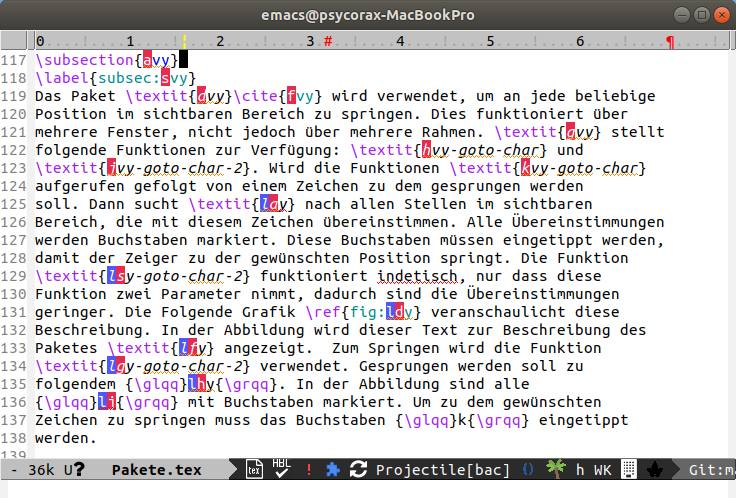
\includegraphics[width=.95\textwidth]{./images/Pakete/avy.png}
  \caption{\label{fig:avy} Das Paket \textit{avy} hat alle gefundenen
    {\glqq}av{\grqq}-Zeichenketten markiert und vorübergehend mit
    anderen Buchstaben überschrieben. Über diese temporären Buchstaben
    ist die gewünschte Zeichenkette erreichbar.}
\end{figure}

\subsubsection{Verwendete Kommandos und Tastenkombinationen}
Das Kommando \textit{avy-goto-char-2} wird an die Tastenkombination
\textbf{M-s} gebunden.\\

\subsection{Ivy}
\label{subsec:ivy}
\textit{Ivy} ermöglicht eine Vervollständigung für Kommandos im
\textit{minibuffer}. Einige dieser Kommandos sind \textit{find-file},
\textit{M-x} und \textit{switch-buffer}. Wird \textit{find-file}
ausgeführt, so zeigt \textit{Ivy} die Dateien und Ordner in dem
aktuellen Verzeichnis an. Wird etwas eingetippt, so werden nur noch
Dateien und Ordner angezeigt, die diese eingetippte Zeichenkette
enthalten. Das Leerzeichen wird als Wildcard interpretiert. Wird zum
Beispiel {\glqq}<SPACE>.tex{\grqq} eingetippt so werden nur noch
tex-Dateien angezeigt. Dies funktioniert bei dem Befehl \textit{M-x}
auch für Funktionen. Die Grafik \ref{fig:ivy} veranschaulicht diese
Beschreibung. In der Abbildung wurde zu einem
\textit{Latex}-Verzeichnis navigiert. In diesem Verzeichnis wird nach
allen Dateien und Ordnern gesucht, welche die Zeichenkette
{\glqq}tex{\grqq} enthalten. \cite{Ivy}\\

\subsubsection{Verwendete Kommandos und Tastenkombinationen}
Das Kommando \textit{ivy-switch-buffer} wird in der
Konfigurationsdatei, welche im Zuge der Arbeit entstanden ist, an die
Tastenkombination \textbf{C-x b} gebunden. Außerdem wird \textit{ivy}
global aktiviert.\\

\begin{figure}[h]
  \centering
  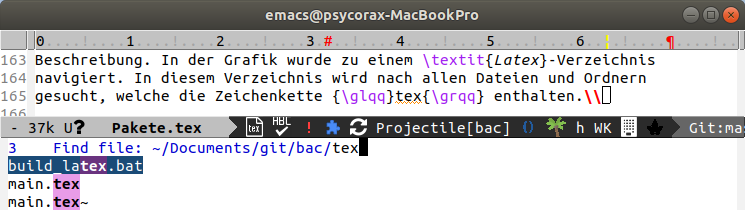
\includegraphics[width=.95\textwidth]{./images/Pakete/ivy.png}
  \caption{\label{fig:ivy} Die verbesserte Suche mit dem Paket
    \textit{ivy} wird in dieser Abbildung dargestellt.}
\end{figure}

\subsection{Swiper}
\label{subsec:swiper}
\textit{Swiper} ist eine Alternative zu
       {\glqq}isearch{\grqq}. \textit{Isearch} ist in Emacs
       standardmäßig enthalten. Das Paket \textit{swiper} verwendet
       \textit{Ivy} um eine Übersicht der Übereinstimmungen im
       \textit{minibuffer} anzuzeigen. Zwischen diesen
       Übereinstimmungen kann mit den Pfeiltasten gesprungen
       werden. Das Leerzeichen dient auch hier als
       Wildcard. \cite{Swiper}\\

\subsubsection{Verwendete Kommandos und Tastenkombinationen}
Das Kommando \textit{swiper} wird in der Konfigurationsdatei, welche
im Zuge der Arbeit entstanden ist, an die Tastenkombinationen
\textbf{C-s} und \textbf{C-r} gebunden.\\

\subsection{Counsel}
\label{subsec:counsel}
\textit{Counsel} erweitert das Paket \textit{Ivy}. Diese Erweiterungen
umfassen das Ersetzen einiger Kommandos. So wird zum Beispiel
\textit{find-file} mit \textit{counsel-find-file} ersetzt. Dadurch
wird dieses Kommando erweitert. Eine solche Erweiterung ist, dass mit
der {\glqq}Del-Taste{\grqq} um ein Verzeichnis zurück gesprungen
wird. Dies erspart das Tippen von {\glqq}../{\grqq}. Ebenso sind
mehrere Optionen verfügbar, welche das Öffnen der Dateien betreffen,
wenn im \textit{minibuffer} die Tastenkombination \textbf{M-o}
gedrückt wird. Eine weiter erwähnenswerte Funktion ist
\textit{counsel-yank-pop}. Diese Funktion ersetzt die Funktion
\textit{yank-pop}, welche standardmäßig einen {\glqq}kill
ring{\grqq}\footnote{\url{https://www.gnu.org/software/emacs/manual/html_node/emacs/Earlier-Kills.html}}
enthält. In diesem \textit{kill ring} werden früher kopierte
Zeichenketten {\glqq}kills{\grqq} abgespeichert. Durch die Verwendung
der Funktion \textit{counsel-yank-pop} wird im \textit{minibuffer}
eine Vorschau dieser Zeichenketten angezeigt. Mit den Pfeiltasten kann
durch diese gespeicherten {\glqq}kills{\grqq} navigiert
werden. \cite{Counsel}\\

\subsubsection{Verwendete Kommandos und Tastenkombinationen}
Folgende Funktionen werden durch die \textit{counsel}-Funktionen in
der Konfigurationsdatei, welche im Zuge der Arbeit entstanden ist,
ersetzt:
\begin{itemize}
\item \textbf{M-x} : \textit{counsel-M-x}
\item \textbf{C-x C-f} : \textit{counsel-find-file}
\item \textbf{M-y} : \textit{counsel-yank-pop}
\end{itemize}

\section{Pakete für die automatische Vervollständigung}
\label{sec:autocomplete}
Für Emacs gibt es zwei {\glqq}große{\grqq} Pakete für die automatische
Vervollständigung von Zeichenketten. Diese sind \textit{auto-complete}
(siehe Abschnitt \ref{subsec:ac}) und \textit{company} (siehe
Abschnitt \ref{subsec:company}). Die Unterschiede sind sehr fein. In
dieser Arbeit werden beide Pakete parallel
verwendet. \textit{Auto-complete} wird für den \textit{org-mode}
verwendet, da es ein zusätzliches Paket für \textit{auto-complete}
gibt, welches spezifisch für den \textit{org-mode} ist. Dieses Paket
hat den Namen \textit{org-ac} (siehe Abschnitt
\ref{subsubsec:orgac}). Es bietet eine verbesserte Vervollständigung
für die Makros des \textit{org-modes}. Für \textit{company} gibt es
kein vergleichbares zusätzliches Paket. \textit{Company} wird hingegen
für alle anderen \textit{major modes} verwendet. Der Grund dafür ist,
dass \textit{auto-complete} beim Ausführen der Standardkonfiguration,
automatisch in jeden \textit{major mode} eingehängt wird. So müsste
\textit{auto-complete} explizit aus jedem \textit{major mode}, in dem
es nicht gebraucht wird, wieder ausgehängt werden. \textit{Company}
ist in Verbindung mit \textit{irony} (siehe Abschnitt
\ref{subsec:irony}) für C++ nur schwer zu umgehen. Auch \textit{Elpy}
(siehe Abschnitt \ref{subsec:elpy}) welches ein Paket für Python ist,
verwendet ebenfalls \textit{company}.\\

\subsection{Auto-Complete}
\label{subsec:ac}
Um \textit{auto-complete} zu verwenden, kann das Kommando
\textit{ac-config-default} aufgerufen werden. Dadurch wird
\textit{auto-complete} für alle \textit{major modes} konfiguriert und
eingehängt. Wird \textit{auto-complete} in einem bestimmten Modus
nicht benötigt, so muss dies explizit eingestellt werden. Wird
\textit{auto-complete} in Verbindung mit \textit{flyspell} (siehe
Abschnitt \ref{subsec:flyspell}) verwendet, so muss das Kommando
\textit{ac-flyspell-workaround} ausgeführt werden. Ansonsten
aktualisieren sich möglichen Vervollständigung nicht
mehr. \cite{AutoComplete}\\

\subsubsection{Org-Ac}
\label{subsubsec:orgac}
\textit{Org-ac} ist eine Vervollständigung für die Makros im
\textit{org-mode}. Ein Vorteil dieses Paketes ist zum Beispiel, dass
bei dem Makro \textit{\#+AUTHOR:} auch automatisch der Name
hinzugefügt wird. Bei \textit{\#+DATE:} wird automatisch das heutige
Datum angefügt. Zum Konfigurieren muss das Kommando nach dem Laden des
Paketes \textit{org-ac/config-default} ausgeführt werden. Dies bindet
den \textit{auto-complete-mode} auch direkt an den
\textit{org-mode}. \cite{OrgAC}\\

\subsection{Company}
\label{subsec:company}
\textit{Company} konfiguriert sich bei der Installation selbst mit den
Standardeinstellungen, hängt sich jedoch nicht in \textit{major modes}
selbstständig ein. Es unterstützt eine Vielzahl an Unterbauten
({\glqq}back-ends{\grqq}). Folgende \textit{back-ends} werden genutzt:
\begin{itemize}
\item CAPF : Unterstützt Vervollständigung von Strukturen in allen
  Programmiersprachen.
\item Elisp : Für die Programmiersprache Emacs Lisp.
\item Clang : Für die Programmiersprache C und C++.
\item ISpell : Für das Paket \textit{flyspell} (siehe Abschnitt
  \ref{subsec:flyspell}).
\item CMake : Für den \textit{cmake-mode} welcher zum Erstellen von
  CMake-Dateien verwendet wird.
\item Yasnippet : Für das Paket \textit{yasnippet} (siehe Abschnitt
  \ref{subsec:yasnippet}).
\item ctags : Ein System zum Taggen (siehe Abschnitt
  \ref{subsec:ctags}).
\item files : Unterstützt Ordner und Dateien, wenn diese in einer
  Datei angegeben werden.
\item keywords : Schlüsselwörter in allen Modi.\\
\end{itemize}
Bei der Konfiguration gibt es einen wichtigen Parameter
(\textit{company-idle-delay}). Wird diese Variable auf null gesetzt,
so vervollständigt \textit{company} ohne Verzögerung. Dies kann bei
leistungsschwachen Rechnern zu Problemen führen. Sollten Probleme
durch \textit{company} auftreten, kann der Wert auf eins abgeändert
werden. Eine weitere verwendete Variable ist
\textit{company-minimum-prefix-length}. Diese bestimmt, ab wie vielen
Zeichen eine Vervollständigung erfolgen soll. \cite{Company}\\

\section{Sonstige Pakete}
\label{sec:misc}
Hier folgen grundlegende Pakete, welche die Benutzung von Emacs
einfacher oder effizienter machen.\\

\subsection{Acewindow}
\label{subsec:acewindow}
Das Paket \textit{ace-window} vereinfacht die Navigation zwischen
Rahmen und Fenstern. Das Kommando \textit{ace-window} ersetzt das
Kommando \textit{other-window}. Das in Emacs standardmäßig enthaltene
Kommando \textit{other-window} wechselt zu Fenstern innerhalb eines
Rahmens in einer definierten Reihenfolge. \textit{Ace-window}
erweitert dies, indem die Fenster in dieser Reihenfolge nummeriert
werden. Sind mehr als zwei Fenster offen, werden bei dem Ausführen des
Kommandos der Inhalt der Fenster {\glqq}schwächer{\grqq}
dargestellt. Im jeweils \textit{oberen linken} Rand befindet sich die
Nummer des Fensters. Über diese Nummer ist nun das jeweilige Fenster
erreichbar. Mit \textit{ace-window} kann auch zu den Fenstern
unterschiedlicher Rahmen gesprungen werden. Die folgende Grafik
\ref{fig:acewindow} veranschaulicht dies. \cite{AceWindow}

\begin{figure}[h]
  \centering
  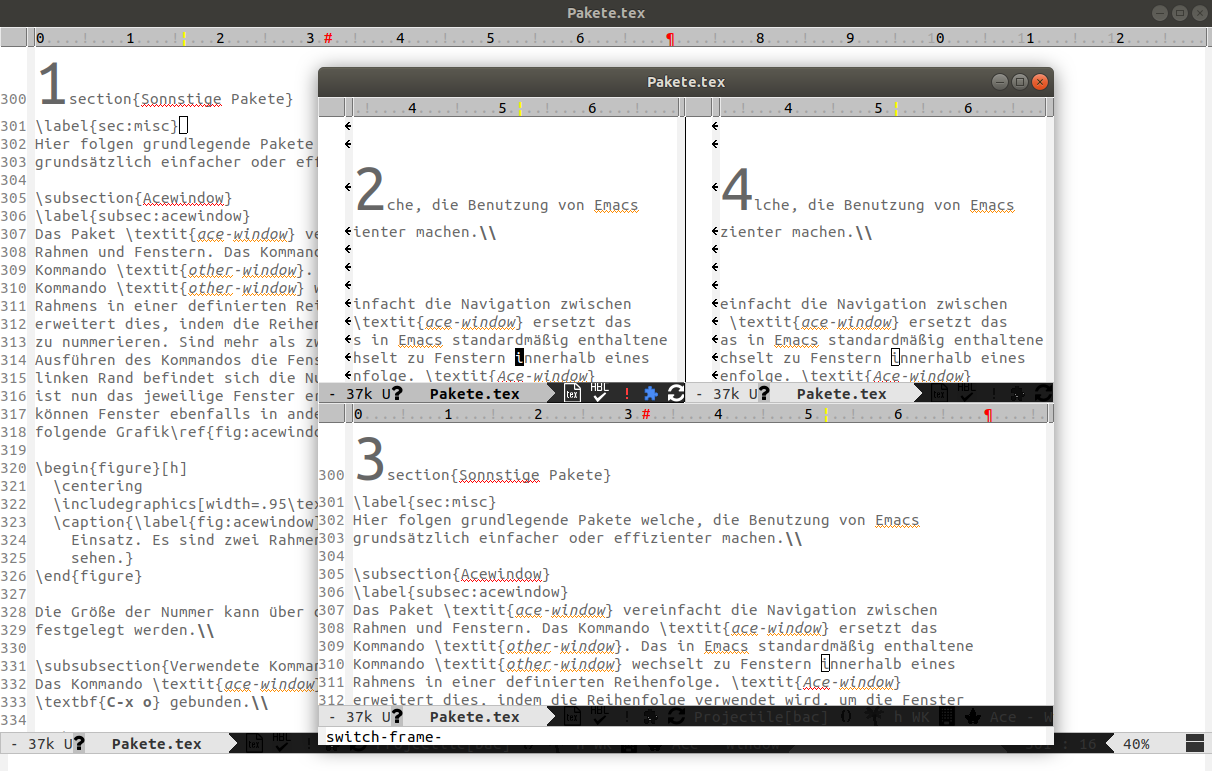
\includegraphics[width=.95\textwidth]{./images/Pakete/acewindow.png}
  \caption{\label{fig:acewindow} Das Paket \textit{ace-window} im
    Einsatz. Es sind zwei Rahmen mit insgesamt vier Fenstern zu
    sehen.}
\end{figure}

Die Größe der dargestellten Nummer kann über den Parameter
\textit{:height} festgelegt werden. Für die Grafik \ref{fig:acewindow}
wurde für \textit{:height} der Wert 4.0 verwendet.\\

\subsubsection{Verwendete Kommandos und Tastenkombinationen}
Das Kommando \textit{ace-window} wird in der Konfigurationsdatei,
welche im Zuge der Arbeit entstanden ist, an die Tastenkombination
\textbf{C-x o} gebunden.\\

\subsection{Try}
\label{subsec:try}
Das Paket \textit{try} wird verwendet, um andere Pakete testen zu
können. Sollte ein neues Paket ausprobiert werden, dann wird einfach
\texttt{M-x try} ausgeführt und in den \textit{minibuffer} wird der
Namen des neuen Pakets getippt. Dadurch wird das Paket für die
aktuelle Sitzung installiert. Bei einem Neustart von Emacs ist das
Paket nicht mehr vorhanden. \cite{Try}\\

\subsection{Which-Key}
\label{subsec:whichkey}
Das Paket \textit{which-key} ist sehr hilfreich für
Emacs-Neulinge. Wird eine Tastenkombination eingetippt welche eine
weitere Eingabe erfordert, so erscheint ein Fenster mit den möglichen
Kombinationen. In der folgenden Abbildung \ref{fig:whichkey} wurde die
Tastenkombination \textbf{C-x} eingetippt. Die Grafik zeigt das
geöffnete \textit{which-key}-Fenster. In dem Fenster sind alle
möglichen Tastenkombinationen zu sehen, inklusive der
Beschreibungen. Diese Beschreibungen erläutern, welche Funktion hinter
den Tastenkombinationen steckt. Mit jeweils \textbf{C-h n} und
\textbf{C-h p} kann durch die Seiten {\glqq}geblättert{\grqq}
werden. Die Zeit nach der dieses \textit{which-key}-Fenster erscheinen
soll, kann über die Variable \textit{which-key-idle-delay} definiert
werden. \cite{WhichKey}\\

\begin{figure}[h]
  \centering
  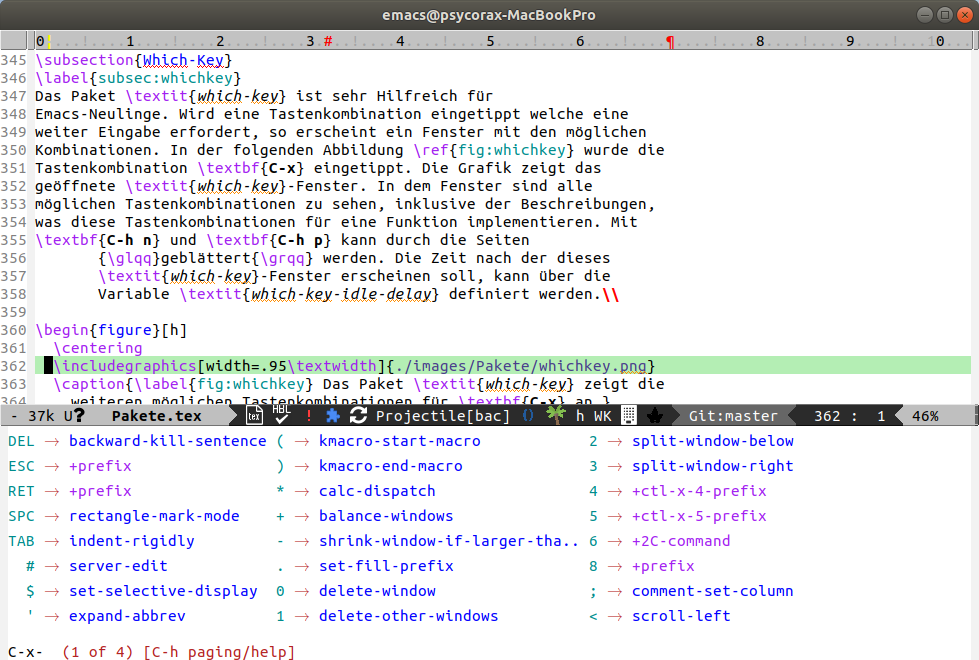
\includegraphics[width=.95\textwidth]{./images/Pakete/whichkey.png}
  \caption{\label{fig:whichkey} Das Paket \textit{which-key} zeigt die
    weiteren möglichen Tastenkombinationen für \textbf{C-x} an.}
\end{figure}

\subsubsection{Verwendete Konfigurationen}
Die Zeit bis das Fenster auftaucht wird in der Konfigurationsdatei,
welche im Zuge der Arbeit entstanden ist, auf eine Sekunde gesetzt.\\

\subsection{Hungry-Delete}
\label{subsec:hungrydelete}
\textit{Hungry-delete} ist ein Paket, mit dem alle aufeinander
folgenden Leerzeichen auf einmal gelöscht werden können. Standardmäßig
ist die Funktionalität \textit{hungry-delete} nur im
\textit{cc-mode}\footnote{\url{https://www.gnu.org/software/emacs/manual/html_mono/ccmode.html}}
implementiert. Das Paket \textit{Hungry-delete} lagert diese
Funktionalität in einen \textit{minor mode} aus. Dadurch kann
\textit{hungry-delete} in allen beliebigen \textit{major modes}
verwendet werden. \cite{HungryDelete}\\

\subsubsection{Verwendete Konfigurationen}
Der \textit{hungry-delete}-Modus wird global aktiviert.\\

\subsection{Expand-Region}
\label{subsec:expandregion}
Das Paket \textit{expand-region} ermöglicht ein schnelles Markieren
von Text. Mit dem ersten Ausführen der Funktion
\textit{er/expand-region}, wird das Wort auf dem sich der Zeiger
befindet markiert. Nun kann mit den folgenden drei Tasten die Region
angepasst werden:
\begin{itemize}
\item \textbf{+} : Erweitert die Region.
\item \textbf{-} : Geht eine Erweiterung zurück.
\item \textbf{0} : Bricht die Funktion ab.
\end{itemize}
Regionen sind anfangs durch das Wort definiert. Weitere Abgrenzungen
der Regionen erfolgt durch Klammern, Hochkomma und
Absätze. \cite{ExpandRegion}\\

\subsubsection{Verwendete Kommandos und Tastenkombinationen}
Die Funktion \textit{er/expand-region} wird an Tastenkombination
\textbf{C-+} gebunden.

\subsection{Multiple-Cursors}
\label{subsec:multiplecursors}
Das Paket \textit{multiple-cursors} ermöglicht es, mehrerer Zeiger auf
einmal steuern zu können. Dadurch kann Text an mehreren Stellen zur
selben Zeit editiert werden. Auf die einzelnen Cursor können auch
Makros angewendet werden. Die wichtigsten Funktionen zum Setzen der
Zeiger sind:
\begin{itemize}
\item \textit{mc/mark-next-like-this} : Es wird eine Übereinstimmung
  vor der markierten Zeichenkette gesucht und mit einem zusätzlichen
  Zeiger markiert.
\item \textit{mc/mark-previous-like-this} : Es wird eine
  Übereinstimmung nach der markierten Zeichenkette gesucht und mit
  einem zusätzlichen Zeiger markiert.
\item \textit{mc/mark-all-like-this} : Es werden alle
  Übereinstimmungen mit der markierten Zeichenkette gesucht und mit
  einem zusätzlichen Zeiger markiert.
\end{itemize}
Sind mehrere Zeiger vorhanden, führen alle Zeiger das selbe
aus. \cite{MultipleCursors}\\\\ Auf der Webseite \textit{Emacs
  Rocks!}\footnote{\url{http://emacsrocks.com/}} wird in dem Video
\textit{Epsiode 13:
  multiple-cursors}\footnote{\url{http://emacsrocks.com/e13.html}} das
Potential von \textit{multiple-cursors} sehr gut veranschaulicht.\\

\subsubsection{Verwendete Kommandos und Tastenkombinationen}
Die Funktionen sind in der Konfiguration mit folgenden
Tastenkombinationen verknüpft:
\begin{itemize}
\item \textbf{C->} : \textit{mc/mark-next-like-this}
\item \textbf{C-<} : \textit{mc/mark-previous-like-this}
\item \textbf{C-M-<} : \textit{mc/mark-all-like-this}
\end{itemize}

\subsection{Flyspell}
\label{subsec:flyspell}
\textit{Flyspell} ist ein integriertes Paket in Emacs und muss nicht
explizit installiert werden. Das Paket dient der Rechtschreibprüfung.
Dadurch können einfache Tippfehler vermieden werden. Eine Überprüfung
der Grammatik ist mit diesem Paket nicht möglich. \cite{Flyspell}\\

\subsubsection{Verwendete Konfigurationen}
Es wird eine Funktion verwendet, welche zwischen den Wörterbüchern
Deutsch und Englisch wechselt. Diese Funktion
\textit{fd-switch-dictionary} wird an die Taste \textbf{<F9>}
gebunden.\\

\subsection{Undo-Tree}
\label{subsec:undotree}
Die Rückgängig- und Wiederholen-Funktion in Emacs sind nicht sehr
leicht Überschaubar, da diese einen kompletten Baum aufbauen
können. Das Paket \textit{undo-tree} implementiert eine grafische
Oberfläche. Dadurch ist es einfacher, den Veränderungen zu folgen,
wenn diese wirr verzweigt sind. Die {\glqq}o{\grqq} stellen die Knoten
dar und das {\glqq}x{\grqq} die aktuelle Position. Ist der
\textit{undo-tree} geöffnet, so kann mit Tasten noch weitere
Funktionalität eingeschaltet werden. Diese möglichen Tasten sind:
\begin{itemize}
\item \textbf{t} : Aktiviert Zeitpunkte, wann die einzelnen Knoten das
  letzte mal besucht wurden.
\item \textbf{d} : Zeigt die Unterschiede der einzelnen Knoten in
  einem zusätzlichen Fenster.
\item \textbf{q} : Verlässt die grafische Anzeige \textit{undo-tree}
  an dem momentan befindlichem Knoten.
\end{itemize}
Die folgende Abbildung \ref{fig:undotree} zeigt das Fenster des
\textit{undo-trees}. \cite{UndoTree}

\begin{figure}[h]
  \centering
  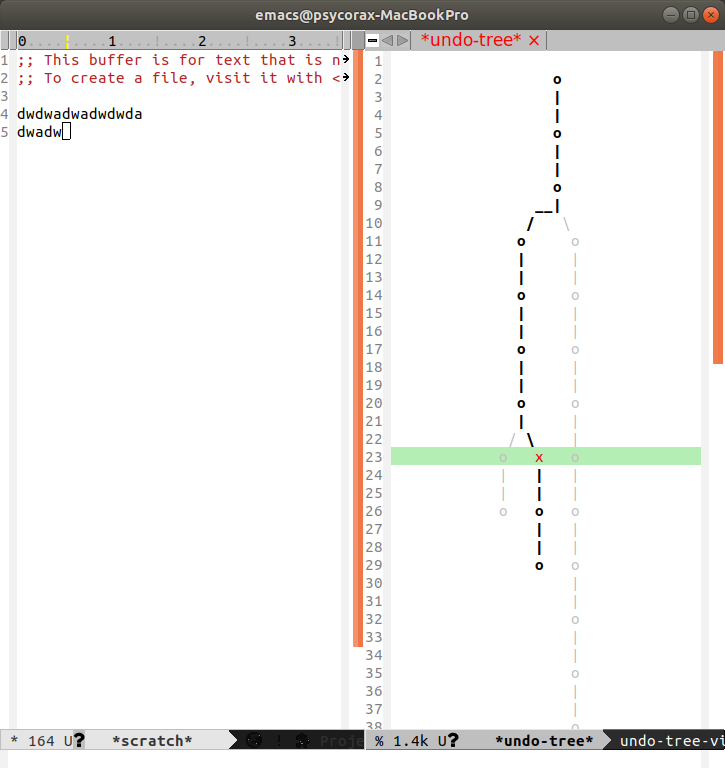
\includegraphics[width=.95\textwidth]{./images/Pakete/undotree.png}
  \caption{\label{fig:undotree} Die Abbildung zeigt das Fenster des
    Paketes \textit{undo-tree}. Es ist keine zusätzliche
    Funktionalität eingeschaltet.}
\end{figure}

\subsubsection{Verwendete Konfigurationen}
Der \textit{undo-tree-mode} wird global aktiviert. Dadurch wird das
\textit{undo-tree}-Fenster bei einem einfach {\glqq}Rückgängig{\grqq}
geöffnet. {\glqq}Rückgängig{\grqq} ist in Emacs standardmäßig an
Tastenkombination \textbf{C-x u} gebunden.\\

\subsection{Smartparens}
\label{subsec:smartparens}
Das Paket \textit{smartparens} fügt bei der Erzeugung einer öffnenden
Klammer sofort auch die schließende Klammer ein. Dabei wird der Zeiger
zwischen den Klammern behalten. Ist etwas markiert, so wird der
markierte Bereich mit Klammern eingeschlossen. Dies funktioniert
ebenso mit Hochkomma. \cite{Smartparens}\\

\subsection{Hydra}
\label{subsec:hydra}
Das Paket \textit{hydra} vereinfacht die Verwendung von
Tastenkombinationen. Es funktioniert in der Verwendung ähnlich wie
\textit{which-key} (siehe Abschnitt \ref{subsec:whichkey}). Eine
\textit{hydra} ist eine Funktionalität, welche mittels Tastendruck
weitere Funktionen über Tastenkombinationen veranschaulicht darstellt
und ermöglicht. Dadurch müssen nicht alle Tastenkombinationen
auswendig gelernt werden. Eine \textit{hydra} wird auf eine
Tastenkombination gebunden, welche beim Ausführen dieser
Tastenkombination in einem Fenster erscheint. In der jeweiligen
\textit{hydra} ist definiert, auf welche Tasten welche Funktionalität
folgt. In dem folgendem Codestück \ref{code:hydra} ist die Definition
einer \textit{hydra} zu sehen. Ganz oben in der ersten Zeile wird der
\textit{hydra} ein Name zugewiesen. Darunter in den Zeilen zwei bis
fünf wird exakt definiert, wie die Darstellung der \textit{hydra} beim
Aufruf aussehen soll. Dies ist in der Abbildung \ref{fig:hydra} zu
sehen. In den Zeilen sechs bis elf werden die einzelnen Tasten der
Funktionalität zugewiesen. Am Ende des Codestücks in den Zeilen 14 bis
15 wird diese \textit{hydra} einer Taste zugewiesen. \cite{Hydra}\\

\begin{program}[h]
  \lstinputlisting[language=Lisp, firstline=1,
    lastline=15]{./code/Pakete/hydra.el}
  \caption{\label{code:hydra}Dieses Codestück zeigt die Definition
    einer \textit{hydra} für den \textit{vhdl-mode}.}
\end{program}

\begin{figure}[h]
  \centering
  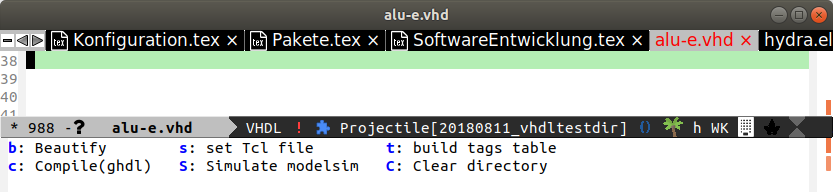
\includegraphics[width=.95\textwidth]{./images/Pakete/hydra.png}
  \caption{\label{fig:hydra} Die geöffnete \textit{hydra} für den
    \textit{vhdl-mode}.}
\end{figure}

\subsubsection{Verwendete Konfigurationen}
In dieser Arbeit wurde fallweise eine \textit{hydra} pro \textit{major
  mode} definiert. Dadurch konnten alle \textit{hydras} der Taste
\textbf{<F8>} zugewiesen werden. So wird bei dem Drücken der F8-Taste
eine für den \textit{major mode} spezifische \textit{hydra}
geöffnet. In der Arbeit wurden \textit{hydras} für folgende
\textit{major modes} festgelegt:
\begin{itemize}
\item org
\item C
\item C++
\item Python
\item VHDL
\end{itemize}
Zu beachten ist, dass \textit{treemacs} (siehe Abschnitt
\ref{subsec:treemacs}) eine eigene Hydra definiert.\\

\subsection{Projectile}
\label{subsec:projectile}
\textit{Projectile} wird zum Erkennen und Festlegen von Projekten
verwendet. Durch \textit{projectile} werden Verzeichnisse welche mit
Versionsverwaltungssystemen verwaltet werden, automatisch als Projekt
erkannt. Zusätzlich erkennt \textit{projectile} Verzeichnisse als
Projekte, wenn eine leere Datei mit dem Namen
{\glqq}.projectile{\grqq} vorhanden ist. Durch die Definition von
Projekten, werden zusätzliche Funktionen für die Suche
bereitgestellt. Diese zusätzlichen Such-Funktionen beschränken sich
auf das aktuelle Projekt. Dadurch kann Zeit gespart
werden. \cite{Projectile}\\

\subsubsection{Verwendete Konfigurationen}
Der \textit{projectile-mode} wird global eingeschaltet. Die
automatische Vervollständigung der \textit{projectile}-Funktionen wird
durch \textit{ivy} (siehe Abschnitt \ref{subsec:ivy}) durchgeführt.\\

\subsection{Magit}
\label{subsec:magit}
Das Paket \textit{magit} implementiert eine komplette Oberfläche für
\textit{Git}. Alle gängigen Kommandos für \textit{git} können mit
diesem Paket einfach ausgeführt werden. Es ist eine Kombination aus
Konsole und grafischer Oberfläche. Die Anzeige erfolgt grafisch, es
kann jedoch alles mit Tastenkombinationen gesteuert werden. Alle
möglichen Tastenkombinationen können mit der Eingabe eines
Fragezeichens angezeigt werden. Dadurch sind alle Kommandos sehr
übersichtlich dargestellt und müssen nicht auswendig gelernt
werden. Dieses Paket ist sowohl für Anfänger als auch erfahrene
\textit{Git}-Benutzer geeignet. \cite{Magit}\\\\ Für eine Einführung
in \textit{magit} wird der folgende Link \cite{MagitGuide}
empfohlen.\\

\subsubsection{Verwendete Konfigurationen}
Das \textit{magit}-Fenster kann mit der Tastenkombination \textbf{C-x
  g} aufgerufen werden. Es werden spezifische Farben für die
Markierungen des Hintergrunds festgelegt. Da sich diese Farben mit dem
in dieser Arbeit verwendeten Farbschema (siehe Abschnitt
\ref{subsec:themes}) besser vertragen.\\

\section{Pakete für grafische Elemente}
\label{sec:gui}
Die folgenden Pakete modifizieren die grafische Oberfläche von
Emacs. Einige dieser Pakete unterstützen auch die Verwendung der
Maus. Im Anhang auf den Seiten \pageref{fig:nogui} und
\pageref{fig:gui} befinden sich zwei Abbildungen von
Emacs-Rahmen. Einmal mit und einmal ohne grafische Elemente. Es wird
bei beiden das Farbschema {\glqq}zenburn{\grqq} (siehe Abschnitt
\ref{subsec:themes}) verwendet.\\

\subsection{Themes}
\label{subsec:themes}
In Emacs sind standardmäßig {\glqq}Farbschemas{\grqq}
(\textit{themes}) enthalten. Diese können einfach mit dem Befehl
\texttt{M-x load-theme} ausgewählt werden. Es gibt auch externe
\textit{themes}, welche von der \textit{Community} zur Verfügung
gestellt werden. Diese werden auf unterschiedlichen
Webseiten\footnote{\url{https://pawelbx.github.io/emacs-theme-gallery/}}
gesammelt. Die meisten \textit{themes} von diesen Seiten können auch
direkt von \textit{melpa} (siehe Abschnitt \ref{sec:paketebasics})
installiert werden.\\

\subsubsection{Verwendete Konfigurationen}
In dieser Arbeit sind zwei externe \textit{themes} konfiguriert. Das
\textit{theme}
       {\glqq}Zenburn\footnote{\url{https://github.com/bbatsov/zenburn-emacs}}{\grqq}
       und das \textit{theme}
       {\glqq}hemisu-dark\footnote{\url{https://github.com/andrzejsliwa/hemisu-theme}}{\grqq}.\\

\subsection{Powerline}
\label{subsec:powerline}
Das Paket \textit{powerline} reorganisiert die \textit{mode line}
(siehe Abschnitt \ref{sec:emacsstart}). Dadurch wird diese Leiste
übersichtlicher dargestellt. Es werden fünf unterschiedliche Schemata
zur Verfügung gestellt nach welchen die Leiste angeordnet werden
kann. Dieses Paket ist im Anhang auf Seite \pageref{fig:gui} in der
Abbildung \ref{fig:gui} im Bereich {\glqq}A{\grqq} zu
sehen. \cite{Powerline}\\

\subsection{Mode-Icons}
\label{subsec:modeicons}
\textit{Mode-icons} ersetzt die Namen der Modi durch Icons in der
\textit{mode line} (siehe Abschnitt \ref{sec:emacsstart}). Die Icons
benötigen viel weniger Platz als die ausgeschriebenen Namen der
Modi. Dadurch ist mehr Platz in der\textit{mode line}, wodurch diese
übersichtlicher erscheint. Werden Modi nicht von dem Paket
\textit{mode-icons} unterstützt, so wird dieser Modus ausgeschrieben
dargestellt. Dieses Paket ist im Anhang auf Seite \pageref{fig:gui} in
der Abbildung \ref{fig:gui} im Bereich {\glqq}B{\grqq} zu
sehen. \cite{ModeIcons}\\

\subsection{Tabbar-Ruler}
\label{subsec:tabbarruler}
Dieses Paket benutzt die Pakete \textit{powerline} (siehe Abschnitt
\ref{subsec:powerline}), \textit{mode-icons} (siehe Abschnitt
\ref{subsec:modeicons}) und \textit{tabbar} (siehe Abschnitt
\ref{subsubsec:tabbar}). Durch das Paket \textit{tabbar-ruler} werden
die Menüleiste, die Symbolleiste und die Leiste mit den Tabs am oberen
Ende des Rahmens versteckt. Wird innerhalb eines Puffers gearbeitet,
so erscheint am oberen Rand ein {\glqq}Lineal{\grqq}. Dieses Lineal
gibt die horizontale Position des Zeigers wieder. Wird der Mauszeiger
an das obere Ende des Rahmen bewegt, so verschwindet das
{\glqq}Lineal{\glqq} und die versteckten Leisten erscheinen. Des
weiteren werden neben den Namen der Tabs die zugehörigen Symbole
angezeigt. Die aufgeklappte Menüleiste und Tableiste ist im Anhang auf
Seite \pageref{fig:gui} in der Abbildung \ref{fig:gui} im Bereich
{\glqq}C{\grqq} zu sehen. \cite{TabbarRuler}\\

\subsubsection{Verwendete Konfigurationen}
In dieser Arbeit ist \textit{tabbar-ruler} folgendermaßen
konfiguriert. Die Tableiste, das Lineal, die Menüleiste und die
Scrollleiste sind aktiviert. Die Symbolleiste ist deaktiviert.\\

\subsubsection{Tabbar}
\label{subsubsec:tabbar}
Dieses Paket erzeugt am oberen Ende des Fensters eine Leiste mit
Tabs. Diese Tabs repräsentieren die offenen Puffer. \cite{Tabbar}\\

\subsection{Org-Bullets}
\label{subsec:orgbullets}
Das Paket \textit{org-bullets} stellt im \textit{org-mode} die
Aufzählungszeichen durch ein beliebiges Zeichen der
\textit{UTF-8-Codetabelle}\footnote{\url{https://www.utf8-zeichentabelle.de/unicode-utf8-table.pl}}
dar. Dadurch sind die Aufzählungen übersichtlicher. Es können auch
mehrere Zeichen definiert werden, damit werden für die
unterschiedlichen Hierarchien unterschiedliche Zeichen
verwendet. Dieses Paket ist im Anhang auf Seite \pageref{fig:gui} in
der Abbildung \ref{fig:gui} im Bereich {\glqq}D{\grqq} zu
sehen. \cite{OrgBullets}\\

\subsubsection{Verwendete Konfigurationen}
Der \textit{org-bullets-mode} wird an den \textit{org-mode}
angehängt. Als Aufzählungszeichen werden Bindestriche {\glqq}-{\grqq}
verwendet, weil Latex mit der Darstellung einiger
\textit{utf-8}-Zeichen Probleme hat.\\

\subsection{Treemacs}
\label{subsec:treemacs}
Dieses Paket implementiert einen grafischen Dateimanager in Emacs. Es
können einzelne Projekte hinzugefügt und entfernt werden. Innerhalb
von Projekten können Dateien umbenannt, erstellt oder gelöscht
werden. Dieser Dateimanager kann auch mit der Maus bedient
werden. Dieses Paket ist im Anhang auf Seite \pageref{fig:gui} in der
Abbildung \ref{fig:gui} im Bereich {\glqq}E{\grqq} zu
sehen. \cite{Treemacs}\\

\subsubsection{Verwendete Konfigurationen}
Es wird die empfohlene
Konfiguration\footnote{\url{https://github.com/Alexander-Miller/treemacs\#installation}}
verwendet. Zusätzlich wird das Öffnen und Schließen von Ordnern und
Dateien von einem Doppelklick mit der Maus, auf einen einfachen Klick
abgeändert\footnote{\url{https://github.com/Alexander-Miller/treemacs\#mouse-interface}}.

\section{Pakete zum Programmieren}
Die folgenden Pakete unterstützen den Benutzer beim Implementieren von
Software in unterschiedlichsten Sprachen.\\

\subsection{Ag}
\label{subsec:ag}
Das Paket \textit{ag} wird zur dateiübergreifenden Suche verwendet. Es
verwendet das Programm
\textit{silversearcher}\footnote{\url{https://github.com/ggreer/the_silver_searcher}}
zur Suche. In der Fußzeile ist ein
Link\footnote{\url{https://github.com/ggreer/the_silver_searcher\#installing}}
zu finden, wo beschrieben wird wie \textit{silversearcher} auf den
gängigsten Betriebssystemen installiert werden kann. \cite{Ag}\\

\subsubsection{Verwendete Kommandos und Tastenkombinationen}
Folgende Tastenkombinationen wurden an diese Funktionieren gebunden:
\begin{itemize}
\item \textbf{M-g s} : \textit{ag}
\item \textbf{M-g p} : \textit{ag-project}
\item \textbf{M-g P} : \textit{ag-project-at-point}
\end{itemize}

\subsection{Dumb-Jump}
\label{subsec:dumbjump}
Das Paket \textit{dumb-jump} ermöglicht Sprünge zu Definitionen von
Labels. Dies funktioniert mit Hilfe des Pakets \textit{ag} (siehe
Abschnitt \ref{subsec:ag}). Es wird bei jedem Sprung erneut eine Suche
gestartet. Aus diesem Grund ist dies eine langsame Methode um zu Tags
zu springen. In kleinen Projekten funktioniert dies jedoch
hervorragend, für große Projekte wird \textit{ctags} (siehe Abschnitt
\ref{subsec:ctags}) empfohlen. \cite{DumbJump}\\

\subsubsection{Verwendete Kommandos und Tastenkombinationen}
Folgende Tastenkombinationen wurden an diese Funktionieren gebunden:
\begin{itemize}
\item \textbf{M-g j} : \textit{dumb-jump-go}
\item \textbf{M-g J} : \textit{dumb-jump-go-other-windo}
\item \textbf{M-g b} : \textit{dumb-jump-back}
\end{itemize}

\subsection{CTags}
\label{subsec:ctags}
\textit{CTags} ist \textit{kein} eigenständiges Paket für
Emacs. \textit{CTags} wird dennoch hier vorgestellt, weil es eine
Ähnlichkeit zu \textit{dumb-jump} (siehe Abschnitt
\ref{subsec:dumbjump}) hat. Es wird ebenfalls zum Springen zu
Definitionen verwendet. Dazu wird jedoch nicht jedes mal das komplette
Projekt durchsucht. \textit{CTags} arbeitet mit einer Tag-Tabelle in
der alle Tags vorhanden sind. Um dies Tabelle erstellen zu können wird
das eigenständige Programm
\textit{ctags}\footnote{\url{https://github.com/universal-ctags/ctags}}
verwendet. Wurde diese Tabelle erzeugt, kann mit eigenen Funktionen zu
den Tags gesprungen werden. \cite{CTags}\\

\subsubsection{Verwendete Kommandos und Tastenkombinationen}
Zum Erzeugen der Tabelle wurden für die Modi C, C++, Python und VHDL
eigene Funktionen geschrieben. Diese Funktionen können über die
jeweiligen \textit{hydras} (siehe Abschnitt \ref{subsec:hydra})
aufgerufen werden. Um zu den Definitionen zu springen, sind die
folgenden Tastenkombinationen definiert:
\begin{itemize}
\item \textbf{M-.} : Springe zu der Definition des markierten Tags.
\item \textbf{M-,} : Springe zurück zu dem Tag wo \textbf{M-.}
  ausgeführt wurde.\\
\end{itemize}


\subsection{Yasnippet}
\label{subsec:yasnippet}
Dieses Paket ermöglicht die Verwendung von Vorlagen, sogenannten
{\glqq}snippets{\grqq}. Es können eigene Vorlagen definiert werden und
es kann ebenfalls das Paket mit dem Namen \textit{yasnippet-snippets}
(siehe Abschnitt \ref{subsec:yasnippetsnippets}) geladen
werden. Dieses Paket enthält eine Vielzahl an vordefinierten
Vorlagen. \cite{Yasnippet}\\

\subsubsection{Verwendete Konfigurationen}
Es wurden im Zuge der Arbeit einige Vorlagen erstellt, diese sind
hier\footnote{\url{https://github.com/Psycorax/emacs/tree/master/mySnipps}}
verfügbar. Der Ordner {\glqq}snippets{\grqq} muss in das Verzeichnis
{\glqq}$\sim$/.emacs.d{\grqq} kopiert werden. Dadurch können diese
Vorlagen verwendet werden.\\

\subsection{Yasnippet-Snippets}
\label{subsec:yasnippetsnippets}
Das Paket \textit{yasnippet-snippets} stellt für alle verwendeten
Haupt-Modi Vorlagen {\glqq}snippets{\grqq} zur Verfügung. Diese
Vorlagen umfassen:
\begin{itemize}
\item Kopfzeilen
\item Fußzeilen
\item Codestücke
\end{itemize}
Diese Vorlagen können auch an die persönlichen Anforderungen angepasst
werden. \cite{YasnippetSnippets}\\

\subsection{Flycheck}
\label{subsec:flycheck}
Dieses Paket überprüft die Syntax des geschriebenen Codes bereits beim
Tippen. Fehler werden direkt im Code markiert oder wenn gewünscht auch
in einem externen Fenster angezeigt. \textit{Flycheck} ersetzt das in
Emacs standardmäßig installierte Paket
\textit{flymake}\footnote{\url{http://flymake.sourceforge.net/}}. \textit{Flymake}
unterstützt standardmäßig nur die vier Programmiersprachen Emacs Lisp,
Ruby, Python und Perl. In dieser Arbeit werden auch die
Programmiersprachen C, C++ und VHDL behandelt. Aus diesem Grund wird
\textit{flycheck} verwendet, welches mehr als 50
Programmiersprachen\footnote{\url{http://www.flycheck.org/en/latest/languages.html\#flycheck-languages}}
unterstützt. \textit{Flycheck} unterstützt Windows offiziell
\textit{nicht}. Nichts desto trotz funktioniert es einwandfrei auf
Windows in Verbindung mit den Programmiersprachen, welche in dieser
Arbeit verwendet werden. \cite{Flycheck}\\

\subsubsection{Verwendete Konfigurationen}
Der \textit{flycheck-mode} wird global aktiviert.\\

\subsection{Irony}
\label{subsec:irony}
Das Paket \textit{irony} enthält den \textit{minor mode}
\textit{irony-mode} für Emacs. Dieser implementiert eine bessere
automatische Vervollständigung für C, C++ und Objective-C. Diese
Verbesserung ist durch einen \textit{irony-server} im Hintergrund
gegeben. Dieser verwendet
\textit{libclang}\footnote{\url{http://clang.llvm.org/doxygen/group__CINDEX.html}}
und \textit{CMake}\footnote{\url{https://cmake.org/}}. Durch die
Verwendung dieses Servers für die automatische Vervollständigung,
versteht \textit{company} (siehe Abschnitt \ref{subsec:company}), dass
die Sprache C, C++ oder Obejctive-C verwendet wird. Die
Vervollständigung ist dadurch \textit{intelligenter}, weil sie direkt
an die Programmiersprache angepasst ist. \cite{Irony}\\

\subsubsection{Vorraussetzungen für die Verwendung von irony}
Um \textit{irony} verwenden zu können, muss \textit{libclang} und
\textit{CMake} auf dem System installiert sein.\\

\subsection{Company-Irony}
\label{subsec:companyirony}
Dieses Paket verbindet die automatische Vervollständigung durch
\textit{company} und \textit{irony-mode}. Dies geschieht, indem dieses
Paket ein \textit{irony} backend für \textit{company}
implementiert. \cite{CompanyIrony}\\

\subsection{Company-irony-c-headers}
\label{subsec:companyironycheaders}
Das Paket \textit{company-irony-c-header} implementiert ein backend
für \textit{company-mode}. Dieses backend ermöglicht eine automatische
Vervollständigung für Header-Dateien. \cite{CompanyIronyCHeaders}\\

\subsection{Elpy}
\label{subsec:elpy}
Das Paket \textit{elpy} implementiert eine komplette
Entwicklungsumgebung für Python. Damit \textit{elpy} funktioniert,
müssen folgende Python-Pakete auf dem System installiert sein:
\begin{itemize}
\item
  \textbf{jedi}\footnote{\url{https://github.com/davidhalter/jedi}} :
  Für eine bessere automatische Vervollständigung, weil durch
  \textit{jedi} die Vervollständigung an die Programmiersprache
  angepasst wird.
\item
  \textbf{flake8}\footnote{\url{http://flake8.pycqa.org/en/latest/}} :
  Für die Überprüfung der Syntax.
\item
  \textbf{autopep8}\footnote{\url{https://pypi.org/project/autopep8/}}
  : Für automatische
  \textit{pep8}\footnote{\url{https://www.python.org/dev/peps/pep-0008/}}
  Formatierung.
\item \textbf{yapf}\footnote{\url{https://github.com/google/yapf}} :
  Für automatische Code-Formatierung, welche die
  \textit{pep8}-Formatierung einhält und den Code zusätzlich
         {\glqq}schön{\grqq} formatiert.
\end{itemize}
Diese Pakete können auf Linux Ubuntu >= 18.10 einfach mit dem Kommando
{\glqq}sudo apt install elpa-elpy{\grqq} installiert werden. Für
Windows müssen diese Python-Pakete einzeln installiert
werden. \cite{Elpy}\\

\chapter{Die Konfiguration}
\label{cha:Konfiguration}
In diesem Kapitel wird auf die einzelne Konfigurationsdateien
eingegangen. Ebenso werden die Unterschiede der Dateien erklärt.

\section{Die Konfigurationsdateien}
\label{sec:konfigurationsdateien}
Als erstes wird die Datei \textit{init.el} (siehe Abschnitt
\ref{sec:initel}) beschrieben. Diese stellt die Basis dar und wird
direkt von Emacs beim Start als erstes geladen. In dieser Datei kann
eine der folgenden Dateien geladen werden:
\begin{itemize}
\item \textit{myinit\_basic.org} (siehe Abschnitt
  \ref{sec:myinitbasic})
\item \textit{myinit\_coding.org} (siehe Abschnitt
  \ref{sec:myinitcoding})
\end{itemize}

Alle Dateien sind auf \textit{github} unter folgendem Link verfügbar:
\url{https://github.com/Psycorax/emacs_bac}

Die Datei \textit{myinit\_basic.org} enthält alle einfachen
Konfigurationen und Pakete. Diese Einstellungen und Pakete
unterstützen den Benutzer beim Editieren und Programmieren. Es werden
nur {\glqq}leichtgewichtige{\grqq} Pakete geladen. Die
Konfigurationsdatei ist für leistungsschwache Rechner ausgelegt. Sie
funktioniert auf allen gängigen Betriebssystemen, auf denen Emacs
läuft.

Die Datei \textit{myinit\_coding.org} enthält alle Einstellungen der
Datei \textit{myinit\_basic.org}. Zusätzlich enthält sie noch weitere
Konfigurationen und Funktionen. Diese Konfigurationen erweitern
einzelne Modi für die Hardware- und Software-Entwicklung. Die
Konfigurationsdatei enthält Pakete für bessere automatische
Vervollständigung, welche spezifisch an die Programmiersprachen
angepasst sind. Es sind Funktionen zum Erstellen von Ordner-Strukturen
für Hardware- und Software-Projekte enthalten, zum Kompilieren und
Debuggen von Software und zum Kompilieren und Simulieren von
VHDL-Code.\\

\section{init.el}
\label{sec:initel}
Wie bereits erwähnt (siehe Abschnitt \ref{sec:konfdatgl}), startet die
Konfigurationen in der Datei \textit{init.el}. Der komplette Inhalt
der Datei ist auf Seite \pageref{code:initel} zu finden. In der ersten
Zeile steht \texttt{(require 'package)}. Dadurch wird überprüft ob das
Paket {\glqq}package{\grqq} bereits vorhanden ist, ist dies nicht der
Fall so wird es installiert. Das Paket \textit{package} implementiert
ein einfaches System zur Verwaltung von Paketen. Dieses
Verwaltungssystem kann Pakete herunterladen und installieren. Die
Pakete werden automatisch auf den aktuellsten Stand gebracht. In Zeile
zwei steht \texttt{(setq package-enable-at-startup nil)}. Diese Zeile
bedeutet, dass die Variable \textit{package-enable-at-startup} auf den
Wert \textit{nil} gesetzt wird. Durch diese Zeile wird ein
Initialisieren der Pakete nach dem Abarbeiten der Datei
\textit{init.el} beim Start verhindert. Die Pakete werden ohnehin in
Zeile neun manuell initialisiert. In den Zeilen drei bis acht werden
externe Archive für Pakete hinzugefügt.  Folgende externen Archive
werden hinzugefügt:
\begin{itemize}
\item \textit{melpa}
\item \textit{melpa-stable}
\item \textit{org-elpa}
\end{itemize}
Das Archiv \textit{melpa} (siehe Abschnitt \ref{sec:paketebasics})
wurde bereits erwähnt. \textit{Melpa-stable} ist ein Archiv in dem
sich nur von Entwicklern als stabil markierte Pakete befinden. Das
dritte Archiv \textit{org-elpa}, wird für die Installation vom
aktuellen \textit{org-mode} (siehe Abschnitt \ref{sec:orgmode})
benötigt. Unter diesen Zeilen befindet sich, in Zeile neun, das
Kommando \texttt{(package-initialize)}. Dieses leitet die manuelle
Initialisierung der Pakete ein. In den Zeilen 11 bis 13 wird das Paket
\textit{use-package} (siehe Abschnitt \ref{subsec:usepackage}) geladen
und installiert. Unterhalb wird das Paket \textit{use-package} bereits
verwendet. Es wird die aktuellere Version von \textit{org}
installiert. Das Kommando in der letzten Zeile (Zeile 19) lädt nun die
weitere Konfigurationsdatei. In dem folgendem Codestück ist dies die
Datei \textit{myinit\_coding.org}. Das Kommando
\texttt{org-babel-load-file} extrahiert alle Codeblöcke von der
\textit{org}-Datei in eine eigene \textit{el}-Datei und diese wird
dann direkt eingebunden.\\

\begin{program}[ht]
\lstinputlisting[language=Lisp, firstline=1,
  lastline=19]{\string~/.emacs.d/init.el}
\caption{\label{code:initel} Die Datei \textit{init.el}.}
\end{program}

Unter diesen 19 Zeilen Code fügt Emacs beim Start automatisch
generierte Variablen hinzu. Diese sollten nicht verändert
werden. Werden sie gelöscht, dann generiert Emacs die Variablen beim
nächsten Start neu.\\

\section{myinit\_basic.org}
\label{sec:myinitbasic}
Diese Konfigurationsdatei kann auf allen gängigen Betriebssystemen auf
denen Emacs läuft verwendet werden. Es werden keine externen Programme
auf dem System benötigt. In der Datei \textit{myinit\_basic.org}
werden ausschließlich {\glqq}leichtgewichtige{\grqq} Pakete
verwendet. Die Datei ist im Anhang \ref{app:basicorg} abgedruckt,
beginnend auf Seite \pageref{app:basicorg}.\\

\subsection{Verwendete Pakete}
\label{subsec:basicverwpak}
Die Pakete, welche in \textit{myinit\_basic.org} verwendet werden:
\begin{itemize}
\item \textit{avy} (siehe Abschnitt \ref{subsec:avy})
\item \textit{ace-window} (siehe Abschnitt \ref{subsec:acewindow})
\item \textit{try} (siehe Abschnitt \ref{subsec:try})
\item \textit{hungry-delete} (siehe Abschnitt
  \ref{subsec:hungrydelete})
\item \textit{multiple-cursors} (siehe Abschnitt
  \ref{subsec:multiplecursors})
\item \textit{flyspell} (siehe Abschnitt \ref{subsec:flyspell})
\item \textit{undo-tree} (siehe Abschnitt \ref{subsec:undotree})
\item \textit{auto-complete} (siehe Abschnitt \ref{subsec:ac})
\item \textit{org-ac} (siehe Abschnitt \ref{subsubsec:orgac})
\item \textit{magit} (siehe Abschnitt \ref{subsec:magit})
\end{itemize}

\subsection{Zusätzliche Konfigurationen}
\label{subsec:basiczuskonf}
Die Konfigurationsdatei besteht nicht nur aus Paketen und deren
Konfigurationen. Es werden auch noch zusätzliche Konfigurationen an
Emacs selbst vorgenommen werden.\\

\subsubsection{Oberfläche}
Dieser Teil erstreckt sich von Zeile 6 bis 46. In diesem Bereich
werden folgende Konfigurationen vorgenommen:
\begin{itemize}
\item Zeile 10 : Es wird die Startseite von Emacs unterdrückt.
\item Zeile 13 : Verstecken der Symbolleiste.
\item Zeile 16 : Ersetzen der Antwortmöglichkeiten von
  {\glqq}yes{\grqq} und {\glqq}no{\grqq} auf {\glqq}y{\grqq} und
  {\glqq}n{\grqq}.
\item Zeile 24 bis 27 : Abhängig von der verwendeten Emacs-Version
  wird ein Modus verwendet um die Zeilennummern am linken Rand der
  Fenster anzuzeigen. Es ist zu beachten dass der Modus
  {\glqq}global-linum-mode{\grqq} bei langen Dateien sehr viel
  Rechenleistung benötigt. Aus diesem Grund wird er auch ab Emacs 26
  durch den effizienteren Modus
  {\glqq}global-display-line-numbers-mode{\grqq} ersetzt.
\item Zeile 36 : Es wird das vorinstallierte Farbschema
  {\glqq}tango-dark{\grqq} geladen.
\item Zeile 42 : Es wird ein Modus eingeschaltet, welcher die ganze
  Zeile in der sich der Zeiger befindet markiert.
\item Zeile 44 : Die Farbe des Zeigers wird dunkelrot gefärbt.
\end{itemize}

\subsubsection{Globale Tastenkombinationen}
Hier befinden sich einige globale Zuweisungen von Tastenkombinationen
auf Kommandos. In Zeile 51 wird der F5-Taste die Funktion
\textit{revert-buffer} zugewiesen. Diese Funktion lädt den aktuellen
Puffer neu von der Festplatte. In Zeile 52 und 53 wird auf die
Tastenkombination \textbf{\textbackslash e\textbackslash ei} das Öffnen der Datei
\textit{myinit\_basic.org} zugewiesen. Zur Erklärung, \textbf{\textbackslash e}
repräsentiert die Esc-Taste. Also entspricht \textbf{\textbackslash e\textbackslash ei} der
Tastenkombination {\glqq}Esc-Taste Esc-Taste i{\grqq}. Das
Schlüsselwort \textit{interactive} verhindert, dass beim Aufruf der
Funktion ein Argument an das Kommando weitergegeben wird.\\

\subsubsection{Puffer}
Für die Verwaltung von Puffern wird \textit{ibuffer} verwendet (Zeile
59). Es wird die Funktion für die standardmäßige Auflistung von
Puffern mit der Auflistung mittels \textit{ibuffer} überschrieben. Die
Auflistung mittels \textit{ibuffer} kategorisiert die offenen Puffer
und verwendet Farben für die Darstellung.\\

\subsubsection{Fenster}
In Zeile 67 wird der Modus
\textit{winner-mode}\footnote{\url{https://www.emacswiki.org/emacs/WinnerMode}}
aktiviert. Dieser ermöglicht es, alte Fensteranordnungen
wiederherzustellen. Der \textit{winner-mode} ist an die
Tastenkombination \textbf{C-c} gefolgt von der Pfeiltaste nach links
und rechts gebunden.\\

\subsubsection{Navigation}
Für die Vervollständigung im \textit{minibuffer} wird der
\textit{ido-mode}\footnote{\url{https://www.emacswiki.org/emacs/InteractivelyDoThings}}
verwendet. Diese Möglichkeiten zur Vervollständigung werden direkt im
\textit{minibuffer} angezeigt. Der \textit{ido-mode} wird statt der
externen Pakete \textit{ivy} (siehe Abschnitt \ref{subsec:ivy}) und
\textit{counsel} (siehe Abschnitt \ref{subsec:counsel}) verwendet. Die
Zeilen 88 bis 91 aktivieren den \textit{ido-mode}.\\

\subsubsection{Org}
In der Zeile 184 wird die Variable \textit{org-hide-leading-stars} auf
{\glqq}true{\grqq} gesetzt. Dadurch wird nur jeweils der letzte Stern
jeder Überschrift angezeigt, wodurch die Auflistung übersichtlicher
wird.\\

\section{myinit\_coding.org}
\label{sec:myinitcoding}
Die Datei \textit{myinit\_coding.org} enthält erweiterte
Konfigurationen, spezifisch für Hardware- und
Software-Entwickler/innen. Diese Datei ist im Anhang
\ref{app:codingorg} ab Seite \pageref{app:codingorg} zu
finden.\\\\ Für folgende Programmiersprachen werden Konfigurationen
vorgenommen:
\begin{itemize}
\item C
\item C++
\item CMake
\item Python
\item Latex
\item VHDL
\item tcl\\
\end{itemize}
Um alle implementierten Funktionen für C und C++ verwenden zu können,
müssen folgende externe Programme auf dem System installiert sein:
\begin{itemize}
\item \textit{CMake}\footnote{\url{https://cmake.org/}}
\item \textit{gdb}\footnote{\url{https://www.gnu.org/software/gdb/}}\\
\end{itemize}
Um alle implementierten Funktionen für Python verwenden zu können,
müssen folgende externe Programme auf dem System installiert sein:
\begin{itemize}
\item \textit{pyinstaller}\footnote{\url{https://www.pyinstaller.org/}}
\item \textit{elpy} (siehe Abschnitt \ref{subsec:elpy})\\
\end{itemize}
Um alle implementierten Funktionen für Latex verwenden zu können,
müssen folgende externe Programme auf dem System installiert sein:
\begin{itemize}
\item \textit{pdflatex}\footnote{\url{https://www.tug.org/texlive/}}\\
\end{itemize}
Um alle implementierten Funktionen für VHDL verwenden zu können,
müssen folgende externe Programme auf dem System installiert sein:
\begin{itemize}
\item
  \textit{Modelsim}\footnote{\url{https://www.intel.com/content/www/us/en/software/programmable/quartus-prime/model-sim.html}}
\item \textit{ghdl}\footnote{\url{https://github.com/ghdl/ghdl}}\\
\end{itemize}

\subsection{Verwendete Pakete}
\label{subsec:codingverwpak}
In dieser Konfigurationsdatei werden alle in dem Kapitel
\ref{cha:pakete} beschriebenen Pakete verwendet.\\

\subsection{Ähnliche Konfigurationen zur Datei init\_basic.org}
Die folgenden Konfigurationen sind denen der Datei
\textit{init\_basic.org} sehr ähnlich. Es werden nur die Unterschiede
beschrieben:
\begin{itemize}
\item Oberfläche : Das Farbschema {\glqq}tango-dark{\grqq} wird in
  dieser Konfiguration nicht verwendet und ist aus diesem Grund
  auskommentiert. Das selbe gilt für die Farbe des Zeigers.
\item Globale Tastenkombinationen : Es wird zusätzlich an die
  Tastenkombination \textbf{C-x o} das Kommando \textit{ace-window}
  global gebunden. Des weiteren werden noch zusätzlich Tasten mit der
  Funktion \textit{find-file} belegt. Dadurch wird ein schnellerer
  Zugriff auf häufig verwendete Dateien ermöglicht.
\item Puffer : Dieser Teil ist identisch.
\item Fenster : Dieser Teil ist ebenfalls identisch.
\item Navigation : Der Modus \textit{ido-mode} wird nicht verwendet,
  da die Pakete \textit{ivy} und \textit{counsel} diesen Modus
  ersetzten.
\end{itemize}

\subsection{Konfigurationen für grafische Elemente}
\label{subsec:guikonf}
In den Zeilen 900 bis 905 der Konfigurationsdatei können grafische
Elemente ein- und ausgeschaltet werden. Es sollte nur ein Farbschema
zur selben Zeit aktiv sein. Eingeschaltet werden die Elemente, wenn
sie auf {\glqq}t{\grqq} gesetzt werden. Ausgeschaltet werden die
Elemente, wenn sie auf {\glqq}nil{\grqq} gesetzt werden.\\

\subsection{Funktionen für die Softwareentwicklung}
\label{subsec:funkswkonf}
In der Konfigurationsdatei \textit{myinit\_coding.org} sind in den
Zeilen 304 bis 320 zwei Funktionen implementiert. Die Funktion
\textit{this-file-in-dir} vergleicht das Verzeichnis der aktuellen
Datei mit dem übergebenen Parameter. Die Funktion
\textit{default-in-dir} vergleicht die gesetzte Variable
\textit{default-directory} mit dem übergebenen Parameter.

In den Zeilen 365 bis 385 ist die Funktion \textit{beautify-me}
definiert. Diese Funktion richtet den Puffer-Inhalt neu aus, löscht
überflüssige Leerzeichen und ersetzt Tabulatoren durch Leerzeichen
oder umgekehrt. Dies ist von dem mitgegebenen Parameter abhängig. Wird
der Parameter \textit{noTabs} auf {\glqq}t{\grqq} gesetzt, so wird die
Funktion \textit{untabify} ausgeführt, andernfalls
\textit{tabify}. Für Emacs Lisp-Code muss die Funktion
\textit{untabify} verwendet werden, sonnst wird die Ausrichtung der
\textit{hydras} verändert. Aus diesem Grund wurde die Funktion
\textit{beautify-el} explizit definiert.\\

\subsection{Der org- und elisp-Modus}
\label{subsec:orgelispmoduskonf}
Es folgen die expliziten Konfigurationen für den \textit{org-mode} und
\textit{emacs-lisp-mode}.

\subsubsection{hydra}
Für den \textit{org-mode} wird eine \textit{hydra} definiert, diese
hat zu diesem Zeitpunkt nur einen Eintrag. Der Eintrag in der
\textit{hydra} verbindet den Buchstaben {\glqq}b{\grqq} mit einer
zusammengesetzten Funktion. Es wird erst die Funktion
\textit{org-edit-special} ausgeführt, danach die Funktion
\textit{beautify-me} mit dem Parameter auf {\glqq}t{\grqq} gesetzt und
als letztes die Funktion \textit{org-edit-src-exit}. Die Funktion
richtet Codeblöcke aus, ohne diese spezifisch öffnen zu müssen.

Für den \textit{emacs-lisp-mode} werden nicht viele Funktionen
benötigt. Hierdurch wird keine \textit{hydra} definiert. An die
Tastenkombination \textbf{C-c C-b} wird die Funktion
\textit{beautify-el} (siehe Abschnitt \ref{subsec:funkswkonf})
gebunden.

\subsubsection{hooks}
In den \textit{org-mode} sind folgende Modi angehängt:
\begin{itemize}
\item \textit{flyspell-mode} (siehe Abschnitt \ref{subsec:flyspell})
\item \textit{smartparens-mode} (siehe Abschnitt
  \ref{subsec:smartparens})\\
\end{itemize}
In den \textit{emacs-lisp-mode} sind folgende Modi angehängt:
\begin{itemize}
\item \textit{smartparens-mode} (siehe Abschnitt
  \ref{subsec:smartparens})
\item \textit{company-mode} (siehe Abschnitt \ref{subsec:company})
\item \textit{yas-minor-mode} (siehe Abschnitt
  \ref{subsec:yasnippet})\\
\end{itemize}

\subsection{Der C- und C++-Modus}
\label{subsec:cc++moduskonf}
Die beiden Modi \textit{c-mode} und \textit{c++-mode} sind für die
Softwareentwicklung in den Sprachen C und C++ ausgelegt. Die folgenden
Konfigurationen werden in der Konfigurationsdatei
\textit{myinit\_coding.org} durchgeführt.\\

\subsubsection{hydra}
Es ist eine \textit{hydra} mit sieben Einträgen definiert. Diese
Einträge verbinden Tasten mit Funktionalitäten:
\begin{itemize}
\item \textbf{b} : Formatierung des Puffers mit Verwendung von
  Tabulatoren.
\item \textbf{u} : Formatierung des Puffers ohne Verwendung von
  Tabulatoren.
\item \textbf{t} : Erstellen einer Datei mit \textit{ctags} (siehe
  Abschnitt \ref{subsec:ctags}).
\item \textbf{d} : Kompilieren des Projektes und Erstellen einer
  ausführbaren Datei zum Debuggen.
\item \textbf{r} : Kompilieren des Projektes und Erstellen einer
  ausführbaren Datei.
\item \textbf{S} : Startet das Debuggen mit
  \textit{gdb}\footnote{\url{https://www.gnu.org/software/gdb/}}.
\item \textbf{C} : Löschen aller generierten Dateien.
\end{itemize}

\subsubsection{hooks}
In den \textit{c-mode} und \textit{c++-mode} sind folgende Modi
angehängt:
\begin{itemize}
\item \textit{smartparens-mode} (siehe Abschnitt
  \ref{subsec:smartparens})
\item \textit{company-mode} (siehe Abschnitt \ref{subsec:company})
\item \textit{yas-minor-mode} (siehe Abschnitt
  \ref{subsec:yasnippet})\\
\end{itemize}

\subsubsection{Funktionen}
In den Zeilen 460 bis 534 sind Funktionen definiert, welche in der
\textit{hydra} den Tasten zugewiesen werden.\\

\subsubsection{Style}
Für die Modi \textit{c-mode} und \textit{c++-mode}, wird die Funktion
{\glqq}set-my-style-cpp{\grqq} definiert. Diese implementiert einen
Programmierstil und wird an die beiden Modi angehängt. Es wird der
vorgegebene Stil {\glqq}stroustrup{\grqq} verwendet und die
Tabulatorweite auf zwei Leerzeichen
abgeändert\footnote{\url{https://www.emacswiki.org/emacs/IndentingC\#toc2b}}.\\

\subsubsection{Optionale Wahl}
In der Zeile 552 kann die Variable \textit{use\_irony} auf
{\glqq}t{\grqq} gesetzt werden, um das Paket \textit{irony} (siehe
Abschnitt \ref{subsec:irony}) mit Erweiterungen zu benutzen. Dadurch
wird eine spezifische automatische Vervollständigung für C und C++
aktiviert.\\

\subsection{Der Python-Modus}
\label{subsec:pythonmoduskonf}
Der Modus \textit{python-mode} ist für die Softwareentwicklung in der
Sprache Python ausgelegt. Die folgenden Konfigurationen werden in der
Konfigurationsdatei \textit{myinit\_coding.org} durchgeführt.\\

\subsubsection{hydra}
Es ist eine \textit{hydra} mit neun Einträgen definiert. Diese
Einträge verbinden Tasten mit Funktionalitäten:
\begin{itemize}
\item \textbf{b} : Formatierung des Puffers mit Verwendung von
  Tabulatoren.
\item \textbf{u} : Formatierung des Puffers ohne Verwendung von
  Tabulatoren.
\item \textbf{t} : Erstellen einer Datei mit \textit{ctags} (siehe
  Abschnitt \ref{subsec:ctags}).
\item \textbf{p} : Starten einer Python-Shell.
\item \textbf{e} : Inhalt des Puffers an die Python-Shell senden und
  ausführen.
\item \textbf{s} : Python-Shell anzeigen.
  \textit{gdb}\footnote{\url{https://www.gnu.org/software/gdb/}}.
\item \textbf{E} : Ausführbare Datei mit \textit{pyinstaller}
  erzeugen.
\item \textbf{Q} : Beenden der Python-Shell.
\item \textbf{C} : Löschen aller generierten Dateien.
\end{itemize}

\subsubsection{hooks}
An den \textit{python-mode} sind folgende Modi angehängt:
\begin{itemize}
\item \textit{smartparens-mode} (siehe Abschnitt
  \ref{subsec:smartparens})
\item \textit{company-mode} (siehe Abschnitt \ref{subsec:company})
\item \textit{yas-minor-mode} (siehe Abschnitt
  \ref{subsec:yasnippet})\\
\end{itemize}

\subsubsection{Funktionen}
In den Zeilen 617 bis 670 sind Funktionen definiert, welche in der
\textit{hydra} den Tasten zugewiesen werden.\\

\subsubsection{Optionale Wahl}
In der Zeile 675 kann die Variable \textit{use\_elpy} auf
{\glqq}t{\grqq} gesetzt werden um das Paket \textit{elpy} (siehe
Abschnitt \ref{subsec:elpy}) zu benutzen.

\subsection{Der Latex-Modus}
\label{subsec:latexmoduskonf}
Der Modus \textit{latex-mode} ist für das Erstellen von Dokumente in
der Sprache Latex ausgelegt. Die folgenden Konfigurationen sind in der
Konfigurationsdatei \textit{myinit\_coding.org} festgelegt.\\

\subsubsection{hydra}
Es ist eine \textit{hydra} mit zwei Einträgen definiert. Diese
Einträge verbinden Tasten mit Funktionalitäten:
\begin{itemize}
\item \textbf{b} : Kompilieren des Latex-Projektes.
\item \textbf{C} : Löschen aller generierten Dateien.
\end{itemize}

\subsubsection{hooks}
An den \textit{latex-mode} sind folgende Modi angehängt:
\begin{itemize}
\item \textit{flyspell-mode} (siehe Abschnitt \ref{subsec:flyspell})
\item \textit{smartparens-mode} (siehe Abschnitt
  \ref{subsec:smartparens})
\item \textit{company-mode} (siehe Abschnitt \ref{subsec:company})
\item \textit{yas-minor-mode} (siehe Abschnitt
  \ref{subsec:yasnippet})\\
\end{itemize}

\subsubsection{Funktionen}
In den Zeilen 715 bis 776 sind Funktionen definiert, welche in der
\textit{hydra} verwendet werden.\\

\subsection{Der VHDL-Modus}
\label{subsec:vhdlmoduskonf}
Der Modus \textit{vhdl-mode} ist für die Hardwarebeschreibungssprache
VHDL ausgelegt. Die folgenden Konfigurationen werden in der
Konfigurationsdatei \textit{myinit\_coding.org} durchgeführt.\\

\subsubsection{hydra}
Es ist eine \textit{hydra} mit sechs Einträgen definiert. Diese
Einträge verbinden Tasten mit folgenden Funktionalitäten:
\begin{itemize}
\item \textbf{b} : Formatierung des Puffers mit dem vorhandenem
  \textit{beautifier}\footnote{\url{http://doc.endlessparentheses.com/Fun/vhdl-beautify-buffer.html}}
  im \textit{vhdl-mode}.
\item \textbf{c} : Kompilieren des Projektes mit \textit{ghdl}.
\item \textbf{s} : Ein \textit{tcl}-Datei festlegen, mit welchem
  \textit{Modelsim} gestartet wird.
\item \textbf{S} : Starten von \textit{Modelsim} mit der gesetzten
  \textit{tcl}-Datei.
\item \textbf{t} : Erstellen einer Datei mit \textit{ctags} (siehe
  Abschnitt \ref{subsec:ctags}).
\item \textbf{C} : Löschen aller generierten Dateien.
\end{itemize}

\subsubsection{hooks}
An den \textit{vhdl-mode} und \textit{tcl-mode} sind folgende Modi angehängt:
\begin{itemize}
\item \textit{smartparens-mode} (siehe Abschnitt
  \ref{subsec:smartparens})
\item \textit{company-mode} (siehe Abschnitt \ref{subsec:company})
\item \textit{yas-minor-mode} (siehe Abschnitt
  \ref{subsec:yasnippet})\\
\end{itemize}

\subsubsection{Funktionen}
In den Zeilen 808 bis 885 sind Funktionen definiert, welche in der
\textit{hydra} den Tasten zugewiesen werden.\\

\subsubsection{Optionale Wahl}
In der Zeile 675 kann die Variable \textit{use\_elpy} auf
{\glqq}t{\grqq} gesetzt werden um das Paket \textit{elpy} (siehe
Abschnitt \ref{subsec:elpy}) zu benutzen.

\chapter{Workflow}
\label{cha:workflow}
Hier wird für die behandelten \textit{major-modes} ein Workflow
vorgeschlagen. Dadurch wird eine schnelle Integration von Emacs in den
Alltag für Hardware- und Software-Entwickler möglich.\\

\section{C und C++}
\label{sec:c++}
Für den \textit{c-mode} und den \textit{c++-mode}, ist der Workflow
identisch. Es gibt zwei Punkte die beachtet werden müssen:
\begin{itemize}
\item Wird ein Projekt in der Programmiersprache C aufgesetzt, müssen
  die Endungen der Dateien von \textit{.cpp} auf \textit{.c}
  abgeändert werden.
\item In der Datei \textit{CMakelists.txt} müssen auch die Dateien
  welche eingefügt werden, von \textit{.cpp} auf \textit{.c}
  abgeändert werden.
\end{itemize}
Der Workflow für den \textit{c++-mode} ist folgendermaßen aufgebaut:
\begin{itemize}
\item Erstellen der Datei \textit{CMakelists.txt}
\item Erzeugen der Projektstruktur
\item Einfügen von Beispielcode in die Datei \textit{main.cpp}
\item Kompilieren des Projektes mit den Flaggen \textit{release} und
  \textit{debug}
\item Debuggen des Projektes
\item Löschen der generierten Dateien
\end{itemize}

\subsection{Aufsetzten und Kompilieren}
\label{subsec:projc++}
Als erstes muss zu dem Verzeichnis navigiert werden, in dem ein
Projekt erstellt werden soll. Hier wird die Datei
\textit{CMakelists.txt} angelegt. Nach dem Öffnen dieser Datei ist zu
erkennen, dass sich Emacs im \textit{cmake-mode} befindet. Nun wird
die Vorlage \textit{cmlists} mit Hilfe des Pakets \textit{yasnippet}
(siehe Abschnitt \ref{subsec:yasnippet}) aufgerufen. Dafür wird
{\glqq}cmlists{\grqq} eingetippt und am Ende die Tabulator-Taste
gedrückt. Es erscheint ein Code-Konstrukt. In dem Code-Konstrukt kann
der Name des Projektes angegeben werden und das Verzeichnis wo sich
die \textit{cpp}-Dateien befinden. Mit der Tastenkombination
\textbf{C-x C-s} wird die Datei abgespeichert. Zum Erstellen der
Ordnerstruktur wird \textbf{M-x mkdir-C-Cpp} ausgeführt. In dem
\textit{minibuffer} wird der gewünschte Name des Projektordners
eingegeben. Die Ordnerstruktur ist erstellt, folgende Ordner sind
erstellt:
\begin{itemize}
\item \textit{doc} : Für jegliche Art von Dokumenten.
\item \textit{inc} : Für alle Header-Dateien.
\item \textit{src} : Für alle Source-Dateien.
\item \textit{tests} : Für Tests.
\end{itemize}
Wurde die Ordnerstrukur erzeugt, so öffnet sich automatisch eine Datei
mit dem Namen \textit{main.cpp}. Hier kann C++-Code eingetippt
werden. Mit der Taste \textbf{<F8>} kann auf die \textit{hydra} (siehe
Abschnitt \ref{subsec:hydra}) für den \textit{c++-mode} zugegriffen
werden. Mit Hilfe der \textit{hydra} werden folgende Funktionen
ausgeführt:
\begin{itemize}
\item \textbf{<F8> b} : Ausrichten des Codes.
\item \textbf{<F8> d} : Kompilieren des Projektes mit der Flagge
  {\glqq}debug{\glqq}.
\item \textbf{<F8> r} : Kompilieren des Projektes mit der Flagge
  {\glqq}release{\glqq}.
\end{itemize}
Sind beim Kompilieren Fehler aufgetreten, müssen diese behoben werden.
Der geöffnete Puffer zeigt die Zeilen an, in denen der Fehler gefunden
wurde. Sind alle Fehler behoben, kann mit Hilfe der \textit{hydra}
(\textbf{<F8> S}), das Debugging (siehe Abschnitt
\ref{subsec:debugc++}) gestartet werden. Durch Eintippen von
    {\glqq}q{\grqq} in der Konsole wird das Debugging beendet. Nun
    werden die generierten Dateien des Projektes gelöscht. Dazu wird
    wiederum die \textit{hydra} verwendet (\textbf{<F8> C}).\\

\subsection{Debugging von C++-Code}
\label{subsec:debugc++}
Nach dem Starten des Debuggings mit der \textit{hydra} (\textbf{<F8>
  S}) öffnet sich
\textit{gdb}\footnote{\url{https://www.gnu.org/software/gdb/}} mit
sechs Fenstern. Die Abbildung \ref{fig:debug} zeigt dies an. Im
Fenster \textit{links oben} ist die \textit{gdb}-Konsole zu sehen. Mit
dieser wird das Debugging gesteuert. Darunter ist die Datei geöffnet,
in welcher sich der Debugger momentan befindet. Die aktuelle Zeile
wird mit einem Pfeil gekennzeichnet. In der Abbildung ist zu erkennen,
dass in der selben Zeile ein Haltepunkt ist. Unterhalb dieses Fensters
befindet sich eine Übersicht, in welcher Datei sich der Debugger
befindet. Auf der Abbildung ist zu sehen, dass sich der Debugger in
Zeile 40 der Datei \textit{Main.cpp} befindet. Im \textit{rechten
  oberen} Fenster werden lokale Variable angezeigt. In diesem Fenster
kann zwischen den lokalen Variablen und den Registern gewechselt
werden. Sollen komplexere Strukturen wie, Listen oder Objekte von
Klassen angezeigt werden. So werden diese in einem zusätzlichen
Fenster angezeigt. Dazu muss sich der Zeiger auf dem gewünschten
Objekt befinden und die Tastenkombination \textbf{C-c C-w} ausgeführt
werden. Es erscheint ein Rahmen mit diesem Ausdruck (zu sehen in
Abbildung \ref{fig:watch}). \textit{Unterhalb} des Fensters mit den
lokalen Ausdrücken befindet sich die Ausgabe auf der Konsole. Unter
dieser befindet sich ein Fenster mit den Haltepunkten. In diesem
Fenster kann zwischen der Anzeige der Haltepunkte und der Anzeige der
laufenden Threads gewechselt werden.\\

\begin{figure}[H]
  \centering
  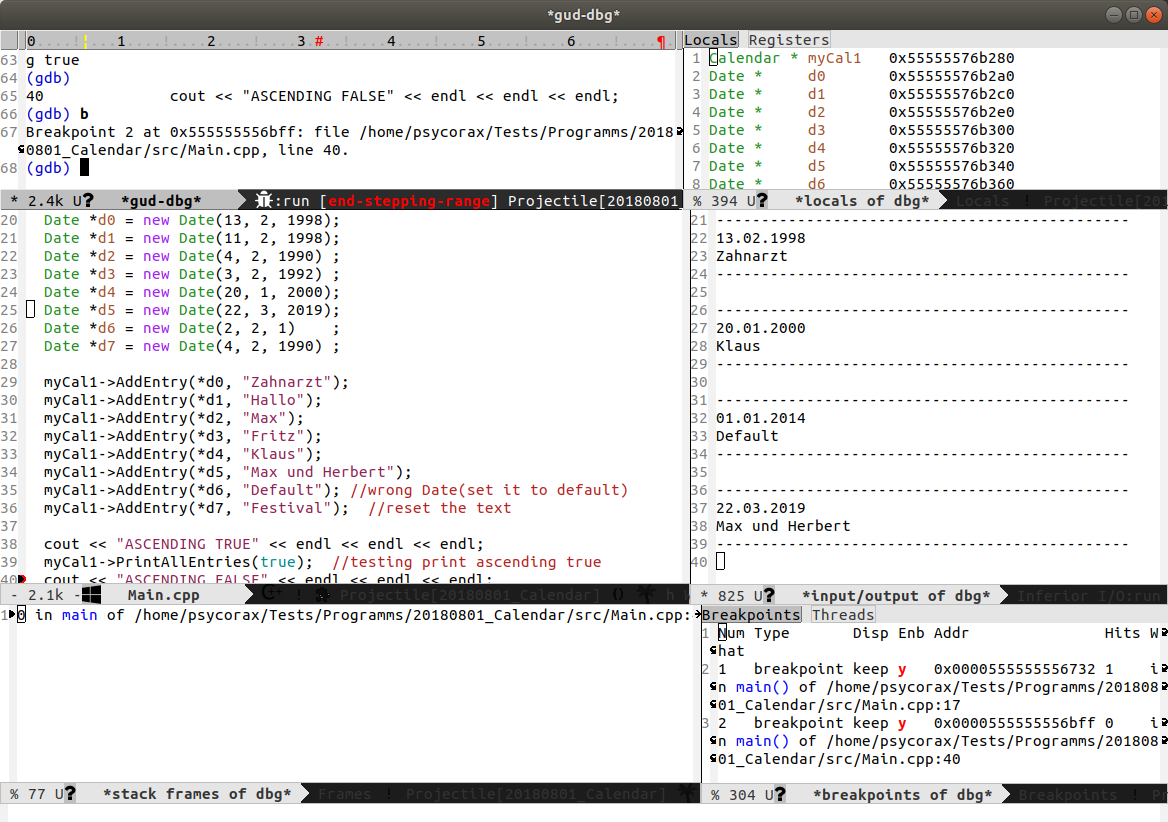
\includegraphics[width=.95\textheight, angle=90]{./images/Workflow/debugversch.png}
  \caption{\label{fig:debug} Das Debuggen in Emacs mit \textit{gdb}.}
\end{figure}

\begin{figure}[H]
  \centering
  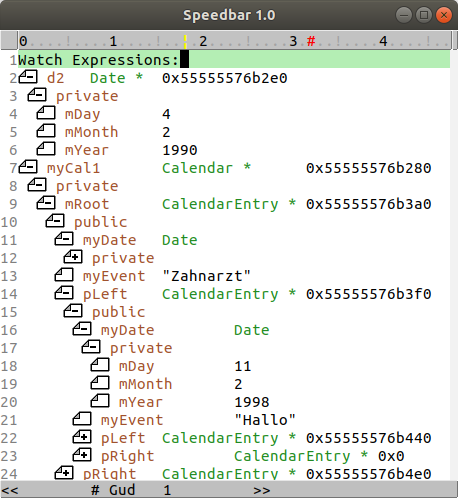
\includegraphics[width=.7\textwidth]{./images/Workflow/watch.png}
  \caption{\label{fig:watch} Diese Abbildung veranschaulicht die
    Darstellung von komplexeren Objekten in Emacs.}
\end{figure}

\section{Python}
\label{sec:python}
Der Workflow für Python ist folgendermaßen aufgebaut:
\begin{itemize}
\item Erstellen der Datei \textit{main.py}
\item Erzeugen der Projektstruktur
\item Einfügen von Beispielcode in die Datei \textit{main.py}
\item Aufruf der Python-Shell und Evaluieren des Codes
\item Wechseln zu der Python-Shell und Beenden der Python-Shell
\item Erzeugen einer ausführbaren Datei
\item Löschen der generierten Dateien
\end{itemize}

\subsection{Aufsetzten und Kompilieren des Projektes}
\label{subsec:projpython}
Als erstes wird zu dem Verzeichnis navigiert, wo das Projekt erstellt
werden soll. Hier wird die Datei \textit{main.py} angelegt. Nach dem
Öffnen dieser Datei ist zu erkennen, dass sich Emacs im
\textit{python-mode} befindet. Um die Ordnerstruktur zu erstellen wird
die Tastenkombination \textbf{M-x mkdir-py} ausgeführt. In dem
\textit{minibuffer} wird der Name des Projektes eingegeben. Nach dem
Erstellen der Ordnerstruktur kann die Datei \textit{main.py} mit Code
beschrieben werden. Für Module ist das Verzeichnis \textit{lib}
vorgesehen. Mit der Taste \textbf{<F8>} kann auf die \textit{hydra}
für den \textit{python-mode} zugegriffen werden. Mit Hilfe der
\textit{hydra} werden folgende Kombinationen ausgeführt:
\begin{itemize}
\item \textbf{<F8> b} : Ausrichten des Codes
\item \textbf{<F8> p} : Starten der Python-Shell
\item \textbf{<F8> e} : Evaluieren des Puffers in der Python-Shell
\item \textbf{<F8> s} : Die Python-Shell anzeigen\\
\end{itemize}
Die Abbildung \ref{fig:python} zeigt einen Puffer mit Python-Code und
unterhalb die Python-Shell, in der dieser Puffer ausgeführt ist. Sind
beim Evaluieren Fehler entstanden, zeigt die Python-Shell die Zeilen
an, an denen sich der Fehler befindet. Sind alle Fehler behoben, kann
mit der Option mit der \textit{hydra} eine ausführbare Datei erstellt
werden (\textbf{<F8> E}). Zum Löschen der generierten Dateien wird
ebenfalls die \textit{hydra} verwendet (\textbf{<F8> C}).\\

\begin{figure}[H]
  \centering
  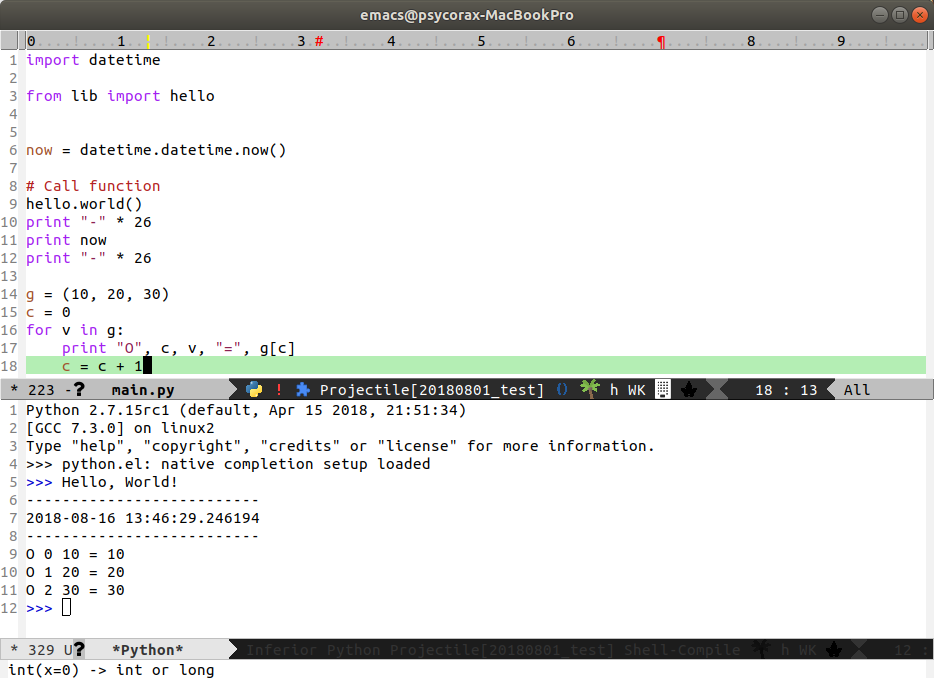
\includegraphics[width=.95\textwidth]{./images/Workflow/pythonshell.png}
  \caption{\label{fig:python} In dieser Abbildung sind ein Puffer mit
    der Datei \textit{main.py} und eine geöffnete Python-Shell zu
    sehen.}
\end{figure}

\section{Latex}
\label{sec:latex}
Der Workflow für Latex ist wie folgt aufgebaut:
\begin{itemize}
\item Erstellen einer Datei mit der Endung \textit{tex}
\item Erzeugen der Projektstruktur
\item Erzeugen der Datei \textit{Definition.tex}
\item Kompilieren des Projektes und erzeugen der \textit{PDF}-Datei
\item Löschen der generierten Dateien
\end{itemize}

\subsection{Aufsetzten und Kompilieren des Projektes}
\label{subsec:prolatex}
Als erstes wird zu dem Verzeichnis navigiert, wo das Projekt erstellt
werden soll. Hier wird eine Datei mit der Endung \textit{tex}
angelegt. Nach dem Öffnen der Datei ist zu erkennen, dass sich Emacs
im \textit{latex-mode} befindet. Nun wird die Vorlage
\textit{baseMain} mit Hilfe des Pakets \textit{yasnippet} (siehe
Abschnitt \ref{subsec:yasnippet}) aufgerufen. Dafür wird
{\glqq}baseMain{\grqq} eingetippt und am Ende der Zeichenkette die
Tabulator-Taste gedrückt. Es erscheint ein Code-Konstrukt, dieses
dient der Vorlage für eine \textit{tex}-Datei. Mit der
Tastenkombination \textbf{C-x C-s} wird die Datei abgespeichert. Zum
Erstellen der Ordnerstruktur wird die \textbf{M-x mkdir-tex}
ausgeführt. In dem \textit{minibuffer} wird der Name des Projektes
eingegeben. Für die Vorlage \textit{baseMain} wird eine zusätzliche
Datei benötigt. Diese Datei enthält die Definitionen. Die Datei
{\glqq}Definition.tex{\grqq} wird erzeugt (\textbf{C-x C-f
  Definition.tex}). Die Vorlage für diese Datei ist mit
\textit{baseDef} erreichbar. Alle benötigten Dateien zum Kompilieren
sind vorhanden. Es wird das Projekt mit der \textit{hydra} für den
\textit{latex-mode} kompiliert und eine PDF-Datei erzeugt
(\textbf{<F8> b}). Ein Fenster erscheint. In diesem sind Warnungen und
Fehler die beim Kompilieren entstanden sind aufgelistet. In der
Abbildung \ref{fig:latex} ist im oberen Fenster der Puffer mit der
\textit{Latex}-Datei zu sehen und unterhalb das Fenster mit den
Warnungen und Fehlern. Sind keine Fehler vorhanden, so wird die
PDF-Datei generiert. Die Tastenkombination \textbf{<F8> C} löscht den
Ordner \textit{build} und damit alle generierten Dateien.\\

\begin{figure}[h]
  \centering
  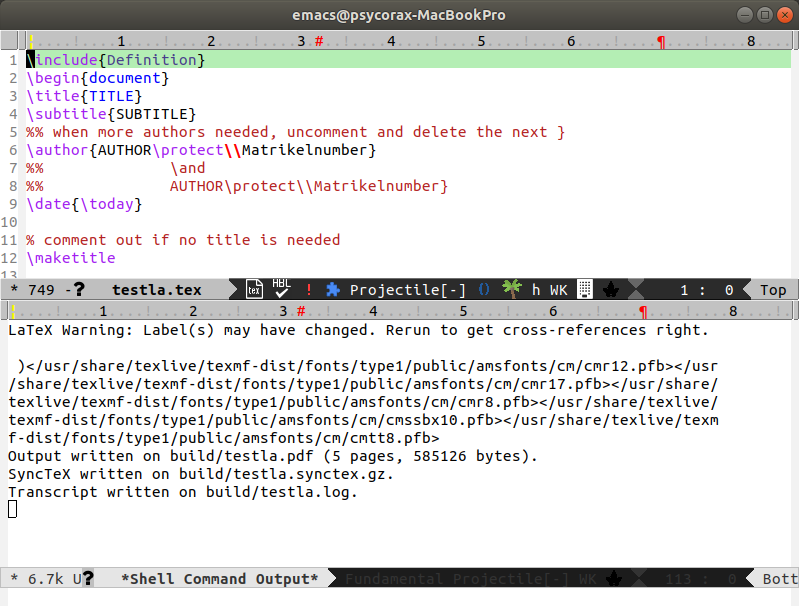
\includegraphics[width=.95\textwidth]{./images/Workflow/latex.png}
  \caption{\label{fig:latex} Kompilieren des \textit{latex}-Projektes.}
\end{figure}

\section{VHDL}
\label{sec:vhdl}
Für den Modus \textit{vhdl-mode} ist der Workflow wie folgt aufgebaut:
\begin{itemize}
\item Erstellen einer Datei mit der Endung \textit{vhd}
\item Erzeugen der Projektstruktur
\item Einfügen von Beispielcode in die \textit{vhd}-Datei
\item Den Code mit
  \textit{ghdl}\footnote{\url{https://github.com/ghdl/ghdl}}
  kompilieren
\item Erzeugen einer \textit{tcl}-Datei
\item Diese \textit{tcl}-Datei zum Start für
  \textit{Modelsim}\footnote{\url{https://www.intel.com/content/www/us/en/software/programmable/quartus-prime/model-sim.html}}
  definieren
\item Starten von \textit{Modelsim} und Ausführen des
  \textit{tcl}-Skriptes
\item Löschen der generierten Dateien
\end{itemize}

\subsection{Aufsetzten und Kompilieren des Projektes}
Als erstes wird zu dem Verzeichnis navigiert, wo das Projekt erstellt
werden soll. Hier wird eine Datei mit der Endung \textit{vhd}
erstellt. Nach dem Öffnen dieser Datei ist zu erkennen, dass sich
Emacs im Modus \textit{vhdl-mode} befindet. Die Projektstruktur wird
erstellt (\textbf{M-x mkdir-vhdl}). In dem Ordner \textit{sim} werden
\textit{tcl}-Datein für das Projekt gesammelt. Eine solche Datei wird
angelegt (\textbf{C-x C-f mysim.tcl}). In der \textit{mode-line} ist
zu erkennen, dass sich Emacs im \textit{tcl-mode} befindet. Nun wird
die Vorlage \textit{tcl} mit Hilfe des Pakets \textit{yasnippet}
(siehe Abschnitt \ref{subsec:yasnippet}) eingefügt. Dafür wird
{\glqq}tcl{\grqq} eingetippt und am Ende der Zeichenkette die
Tabulator-Taste gedrückt. Es erscheint ein Code-Konstrukt, welches als
Vorlage für \textit{tcl}-Dateien zum Kompilieren und Simmulieren
mittels \textit{modelsim} dient. Nachdem alle Dateinamen korrekt
eingefügt sind, wird die Datei abgespeichert (\textbf{C-x C-s}). Der
\textit{src}-Ordner ist für die \textit{vhd}-Dateien vorgesehen. Mit
der \textit{hydra} für den \textit{vhdl-mode} werden folgende
Funktionen ausgeführt:
\begin{itemize}
\item \textbf{<F8> b} : Ausrichten des Codes
\item \textbf{<F8> c} : Kompilieren mit Hilfe von \textit{ghdl}
\item \textbf{<F8> s} : Festlegen der verwendeten\textit{tcl}-Datei
  für \textit{Modelsim}
\item \textbf{<F8> S} : Starten von \textit{Modelsim} und Ausführen
  des \textit{tcl}-Skriptes\\
\end{itemize}
Beim Kompilieren mit \textit{ghdl} kann die Syntax für den momentan
angezeigten Puffer überprüft werden (in Abbildung \ref{fig:ghdl} zu
sehen). Die Simulation mit \textit{Modelsim} basiert auf dem
definierten \textit{tcl}-Skript. Zum Löschen der generierten Dateien
wird die \textit{hydra} verwendet (\textit{<F8> C}).\\

\begin{figure}[h]
  \centering
  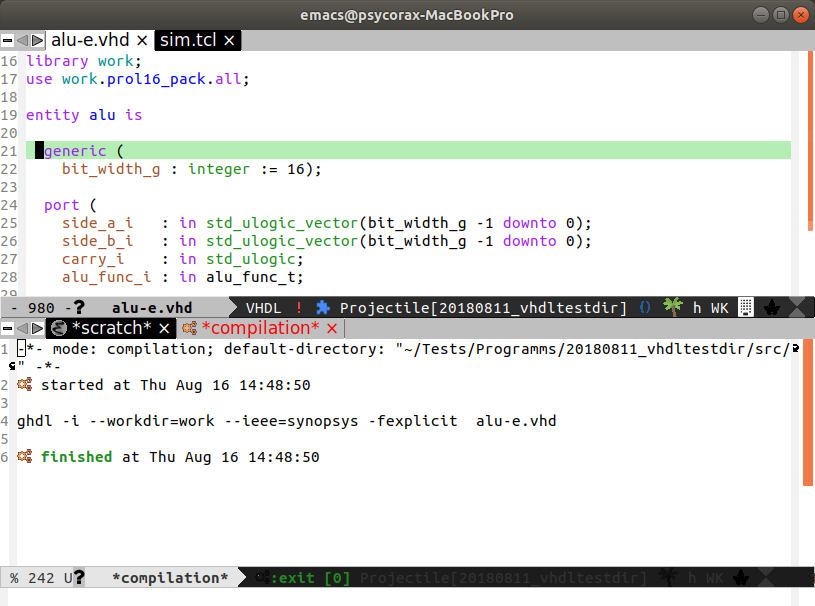
\includegraphics[width=.95\textwidth]{./images/Workflow/ghdl.png}
  \caption{\label{fig:ghdl} Kompilieren des Puffers mit \textit{ghdl}.}
\end{figure}

\chapter{Zusammenfassung}
\label{cha:Zusammenfassung}
\section{Aufgetretene Probleme}
\label{sec:probleme}
Anfangs wurden für die Arbeit Pakete evaluiert, welche ganze
Entwicklungsumgebungen für C und C++ implementieren. Zum Beispiel das
Paket
\textit{cmake-ide}\footnote{\url{https://github.com/atilaneves/cmake-ide}}. Diese
kompletten Entwicklungsumgebungen funktionieren grundsätzlich sehr
gut. Das Problem an diesen fertigen Entwicklungsumgebungen ist, dass
sie meist eine große Anzahl an externen Programme benötigen. Ein
weiteres Problem ist, dass diese Pakete für die unterschiedlichen
Sprachen auf einer Vielzahl an Paketen basieren. Diese Pakete
implementieren meist jedoch grundlegend die selbe Funktionalität.

Die Schwierigkeit bestand nun darin, Pakete zu finden, welche für alle
verwendeten Sprachen verwendet werden können. Diese Pakete sollten
ausschließlich Software verwenden, welche auf mehreren
Betriebssystemen verfügbar ist.

\section{Umsetzung}
\label{sec:umsetzung}
Das Ziel dieser Arbeit war es, einfache Entwicklungsumgebungen für
Emacs zu finden. Diese Entwicklungsumgebungen sollten für mehrere
Programmiersprachen (C, C++, Python, Latex, CMake, Emacs Lisp und
VHDL) parallel verwendbar sein. Die Entwicklungsumgebungen für die
unterschiedlichen Sprachen sollten ähnlich bedienbar sein und auf den
selben Paketen aufsetzten.

Um diese einfachen und ähnlich bedienbaren Entwicklungsumgebungen
realisieren zu können, wurden eigene Funktionen für die einzelnen Modi
definiert. Diese Funktionen bauen auf den gewählten Paketen auf und
erweitern diese. Es wurde folgende Funktionalität implementiert:
\begin{itemize}
\item Die Erstellung von Projekverzeichnissen,
\item Die Ausrichtung und Formatieren von Code,
\item Das Kompilieren des Projektes,
\item Das Erzeugen von ausführbaren Dateien,
\item Das Aufräumen von Projekten, durch entfernen generierter Ordner
  und Dateien,
\item Das Starten des Debuggens für Projekte und
\item Das Starten von Simulationen in externer Software.\\
\end{itemize}
Damit diese Funktionen für den Benutzer leicht zugänglich sind, werden
sie in \textit{hydras} (siehe Abschnitt \ref{subsec:hydra})
hinterlegt.

\section{Mögliche Erweiterungen}
\label{sec:erweiterungen}
Eine mögliche Erweiterung dieser Arbeit ist das Einbinden von Paketen,
welche spezifisch für die Entwicklung auf eingebetteten Systeme
ausgelegt sind. Ein mögliches Paket an dem angesetzt werden kann ist
\textit{stm32-emacs}\footnote{\url{https://github.com/SL-RU/stm32-emacs}}. Dieses
Paket baut beinahe ausschließlich auf Software auf, welche bereits für
die Pakete in dieser Arbeit benötigt wurden.


%%%----------------------------------------------------------
\appendix                                            % Anhang 
%%%----------------------------------------------------------

\chapter{Abbildungen}
\label{cha:abbildungen}

\begin{figure}[ht]
  \centering
  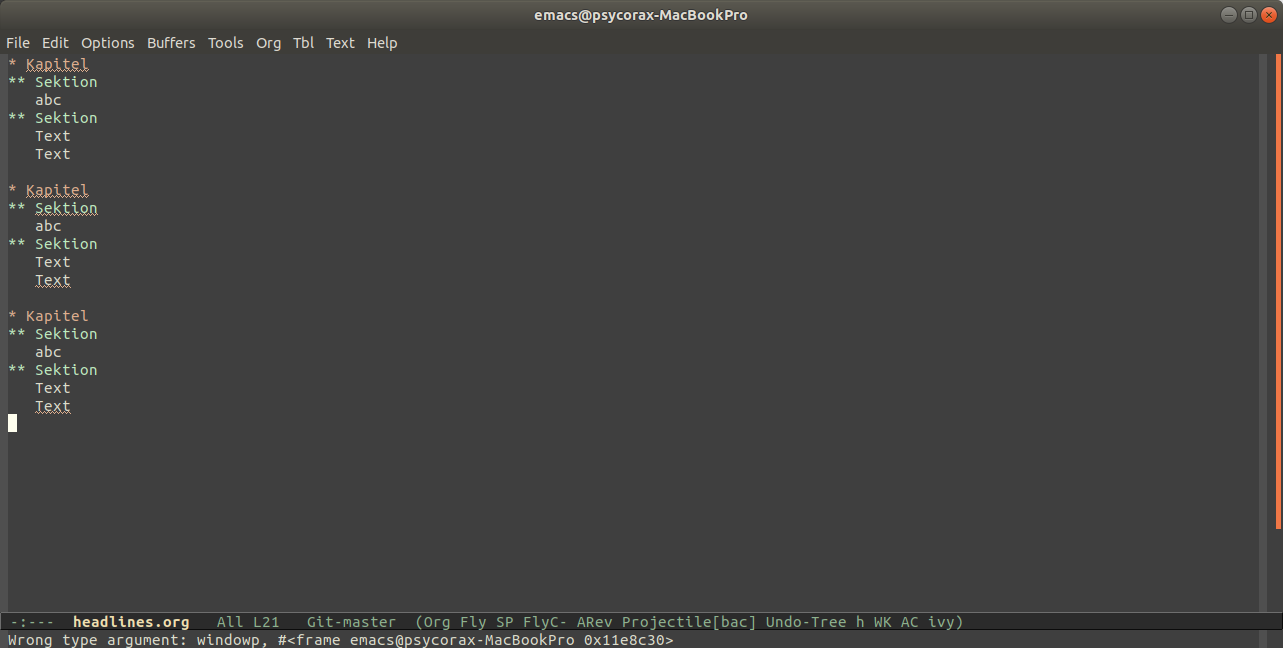
\includegraphics[width=1\textheight, angle=90]{./images/Pakete/nogui.png}
  \caption{\label{fig:nogui} Diese Abbildung zeigt einen Emacs Rahmen
    ohne grafischen Elementen.}
\end{figure}

\begin{figure}[ht]
  \centering
  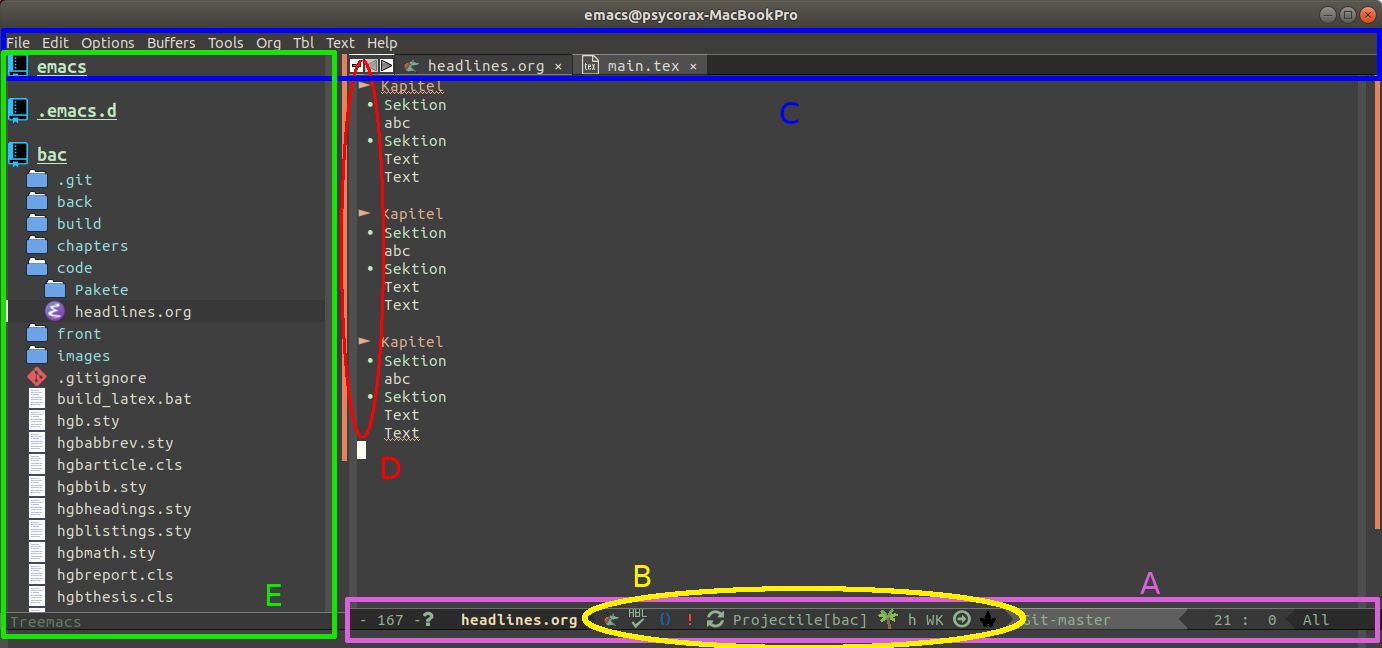
\includegraphics[width=1\textheight, angle=90]{./images/Pakete/gui.png}
  \caption{\label{fig:gui} Diese Abbildung zeigt einen Emacs Rahmen
    mit grafischen Elementen.}
\end{figure}
 % Abbildungen
\chapter{myinit\_basic.org}
\label{app:basicorg}

\lstinputlisting[language=Lisp]{./code/Konfigurationsdateien/myinitbasic.org}
 % myinitbasic.org
\chapter{myinit\_coding.org}
\label{app:codingorg}

\lstinputlisting[language=Lisp]{./code/Konfigurationsdateien/myinitcoding.org}
 % myinitcoding.org
\chapter{Inhalt der CD-ROM/DVD}
\label{app:cdrom}

\paragraph{Format:} 
		CD-ROM, Single Layer, ISO9660-Format%

\section{PDF-Dateien}
\begin{FileList}{/}
%\fitem{_DaBa.dvi} Gesamtdokument (DVI-File, ohne Grafiken)
\fitem{_thesis_reisinger.pdf} Bachelorarbeit %
\end{FileList}

\section{Text-Dateien}
\begin{FileList}{/}
\fitem{_thesis_reisinger_kurzfassung.txt} Kurzfassung %
\fitem{_thesis_reisinger_abstract.txt} Abstract %
\end{FileList}

\section{LateX-Projekt}

\begin{FileList}{/}
\fitem{_thesisReisinger} Ordner mit dem LateX-Projekt %
\end{FileList}

\section{Sonstiges}

\begin{FileList}{/_thesisReisinger/images}
\fitem{*.png} Originalbilder %
\end{FileList}

\section{Sourcedateien}

\begin{FileList}{/}
  \fitem{_emacs_bac} Ordner mit Sourcedateien %
\end{FileList}
 % CD-Inhalt

%%%----------------------------------------------------------
\MakeBibliography                        % Quellenverzeichnis
%%%----------------------------------------------------------

%%% Messbox zur Druckkontrolle ------------------------------
\chapter*{Messbox zur Druckkontrolle}



\begin{center}
{\Large --- Druckgröße kontrollieren! ---}

\bigskip

\calibrationbox{100}{50} % Angabe der Breite/Hoehe in mm

\bigskip

{\Large --- Diese Seite nach dem Druck entfernen! ---}

\end{center}



%%%----------------------------------------------------------
\end{document}
%%%----------------------------------------------------------
